\documentclass[abstract=on]{scrreprt}
%\documentclass[abstract=on]{book}
%https://en.wikibooks.org/wiki/LaTeX/Document_Structure

%---------------- lagt til mal -------------------
\usepackage{amsmath}%math env++
\usepackage{bm}%bold math for vectors
\usepackage{amssymb}%for other math symbols
\usepackage[section]{placeins}%forhindrer floats over sections

%--------------- Tilhørende mal ------------------
\usepackage[utf8]{inputenc}
\usepackage{hyperref}
\usepackage{url}
\usepackage{listings}
\usepackage{enumitem}
\usepackage{setspace}
\usepackage[sort=def, nonumberlist, nopostdot]{glossaries}
\usepackage{natbib}
\usepackage{graphicx}
\usepackage{geometry}
\usepackage{pdflscape}
\usepackage{caption}
\usepackage{multirow}
\usepackage{float}
\usepackage{caption}
\usepackage{subcaption}
\usepackage{tikz}
\usepackage{wrapfig}
\usepackage{chngcntr}
\usepackage{comment}
\usepackage[toc, page]{appendix}
\usepackage{titlesec}

% spacing: how to read {12pt plus 4pt minus 2pt}
%           12pt is what we would like the spacing to be
%           plus 4pt means that TeX can stretch it by at most 4pt
%           minus 2pt means that TeX can shrink it by at most 2pt
%       This is one example of the concept of, 'glue', in TeX
\titlespacing\section{0pt}{10pt plus 4pt minus 2pt}{0pt plus 2pt minus 2pt}
\titlespacing\subsection{0pt}{8pt plus 4pt minus 2pt}{0pt plus 2pt minus 2pt}

\makeatletter
\g@addto@macro{\UrlBreaks}{\UrlOrds}
\makeatother

\renewcommand{\abstractname}{} 
\renewcommand{\glossarysection}[2][]{}
\newcommand{\heart}{\ensuremath\heartsuit}

\lstset{basicstyle=\ttfamily}

% paragraph indentation
\setlength{\parindent}{0em} 

% paragraph spacing
\setlength{\parskip}{1.2em}

% table cell spacing
\setlength{\tabcolsep}{1em}
\renewcommand{\arraystretch}{1}

% list spacing
\setitemize[0]{leftmargin=1.5em, itemsep=-0.5em, topsep=-0.4em}

% normal line spacing
\renewcommand{\baselinestretch}{1.1}

 % Next level after subsection
 \newcommand{\paragraphsection}[1]{\paragraph{#1}\mbox{}\\[0.2cm]}
 \renewcommand*{\glossaryname}{Other}
 
\RedeclareSectionCommand[beforeskip=2\baselineskip, afterskip=1\baselineskip]{chapter}


\makeatletter
\renewcommand{\@chapapp}{}% Not necessary...
\newenvironment{chapquote}[2][2em]
  {\setlength{\@tempdima}{#1}%
   \def\chapquote@author{#2}%
   \parshape 1 \@tempdima \dimexpr\textwidth-2\@tempdima\relax%
   \itshape}
  {\par\normalfont\hfill--\ \chapquote@author\hspace*{\@tempdima}\par\bigskip}
\makeatother

\newcommand{\doubleSignature}[3]{
\vspace{1.5cm}

\noindent
\begin{tabular}{lcl}
    \rule{5cm}{1pt} & \hspace{2cm} & \rule{5cm}{1pt} \\
    #2 & & #3
\end{tabular}
}

\newcommand{\singleSignature}[2]{
\vspace{1.5cm}

\noindent
\begin{tabular}{l}
    \rule{5cm}{1pt} \\
    #2
\end{tabular}
}

\definecolor{dkgreen}{rgb}{0,0.6,0}
\definecolor{gray}{rgb}{0.5,0.5,0.5}
\definecolor{mauve}{rgb}{0.58,0,0.82}

\lstdefinelanguage[mips]{java}%
{morestring=[b]",
morekeywords=[1]{},%
comment=[l]\//%
}[keywords,comments,strings]

\lstset{ %
  basicstyle=\scriptsize,       % the size of the fonts that are used for the code
  basicstyle=\ttfamily,
  numbers=left,                   % where to put the line-numbers
  numberstyle=\tiny\color{gray},  % the style that is used for the line-numbers
  stepnumber=1,                   % the step between two line-numbers. If it's 1, each line 
                                  % will be numbered
  numbersep=5pt,                  % how far the line-numbers are from the code
  backgroundcolor=\color{white},  % choose the background color. You must add \usepackage{color}
  showspaces=false,               % show spaces adding particular underscores
  showstringspaces=false,         % underline spaces within strings
  showtabs=false,                 % show tabs within strings adding particular underscores
  frame=single,                   % adds a frame around the code
  rulecolor=\color{white},        % if not set, the frame-color may be changed on line-breaks within not-black text (e.g. commens (green here))
  tabsize=4,                      % sets default tabsize to 2 spaces
  captionpos=b,                   % sets the caption-position to bottom
  breaklines=true,                % sets automatic line breaking
  breakatwhitespace=false,        % sets if automatic breaks should only happen at whitespace
  title=\lstname,                 % show the filename of files included with \lstinputlisting;
                                  % also try caption instead of title
  keywordstyle=\color{blue},          % keyword style
  commentstyle=\color{dkgreen},       % comment style
  stringstyle=\color{mauve},         % string literal style
  escapeinside={\%*}{*)},            % if you want to add a comment within your code
  morekeywords={*,...}               % if you want to add more keywords to the set
}

\renewcommand{\bibname}{References}

% Edit the meta.tex file to change title, group number and author names 
% Fill in the report title, group number and student names here
\newcommand{\mytitle}{Energy consumption of a GPS}
\newcommand{\myauthor}{Jared Showatatek}

\title{\mytitle}
\author{\myauthor}
\date{\today}



\begin{document}
% Caps roman numbers: \pagenumbering{roman} 
\pagenumbering{roman}
% The title page, edit if you want to customize it 

\begin{titlepage}
\begin{center}

 
% Upper part of the page
~\\[0.5cm]

\includegraphics[height=2.0cm]{Images/NTNU_logo.pdf}\\[1cm]  

% Set the title of the Document between two horizontal lines
\hrule ~\\[0.2cm]
{\huge \bfseries \mytitle}\\[0.4cm]		% print the title of the document
\hrule ~\\[1.5cm]

% Additional Information about the document
\begin{minipage}{1\textwidth}
    \centering
	\large
	By
		\myauthor
\end{minipage}

\vfill
{\large \today}
~\\[0.5cm]

% Bottom of the page

\end{center}
\end{titlepage}

% Main matter - edit corresponding file under content/ to change


\begin{minipage}{\textwidth}
\center\Large{Project Assignment:}\\
\end{minipage}
~\\[2cm]
\begin{minipage}{0.8\textwidth}

	\Large Candidate Name: Jared Showatatek\\ 
	\Large Assignment title: Energy consumption of a GPS\\ 
	\Large Assignment text: Model the energy consumption of a GPS\\
	\Large  Co-supervisor: Kjetil Svarstad\\
	\Large Supervisor: Frank Kraemer\\
	
\end{minipage}
\chapter*{Abstract}



\newpage
%%Preface. Here you can describe the process that led to the writing of this report (i.e., the project work process). Here you can mention why you chose this assignment and specific challenges you met with during your work. You can also thank people for help and support during this project.%%%
%%%%%%%%%TOC%%%%%%%%%%%%%%%%%%%%%%%%%%%%%%%%%%%%%%%%%%%%%%%%%%%%%%%%%%%%%%%%%%%%%%%%%%%%%
\tableofcontents
\newpage
\listoffigures
\listoftables
\lstlistoflistings

\newpage

%%%%%%%%%%%%%%%%%%%%%%%INNLEDNING%%%%%%%%%%%%%%%%%%%%%%%%%%%%%%%%%%%%%%%%%%%%%%%%%%%%%%%%
%%%%%%This is normally Chapter 1 and gives an overview of the assignment and why this work is important. If you have chosen to focus mainly on a part of the assignment text, you may write something about this here and explain why. You also normally give a short description of the structure of the rest of the report towards the end of this chapter.  It is important to indicate which parts that are based on your own work. You may even include a list of your main contributions. %%%%%

\chapter{Introduction}
\pagenumbering{arabic}


%%%%%Introduksjon, GPS i IOT verden osv%%%%%%%

Internet of things (IoT) is the network which consists of objects that are connected to the internet such as sensors, vehicles, actuators and other embedded devices. The objects uses the internet to deliver data or be controlled remotely throughout the Internet. IoT is used in the industry to improve the efficiency of operations, safety and security and give valuable insights in analyzing data. The use cases for IoT is also relevant for the general consumer as more of the objects in the household are connected to the Internet. Two examples are: Controlling the oven temperature with a mobile app or notifying the hospital if a irregular heart rhythm is noticed by the person's pacemaker. IoT is one of the fastest growing trends in technology today, which is highlighted by Gartners Hype cycle of 2017 shown in figure \ref{fig:Gartner}\\


\begin{minipage}[t]{0.8\textwidth}
    \centering
    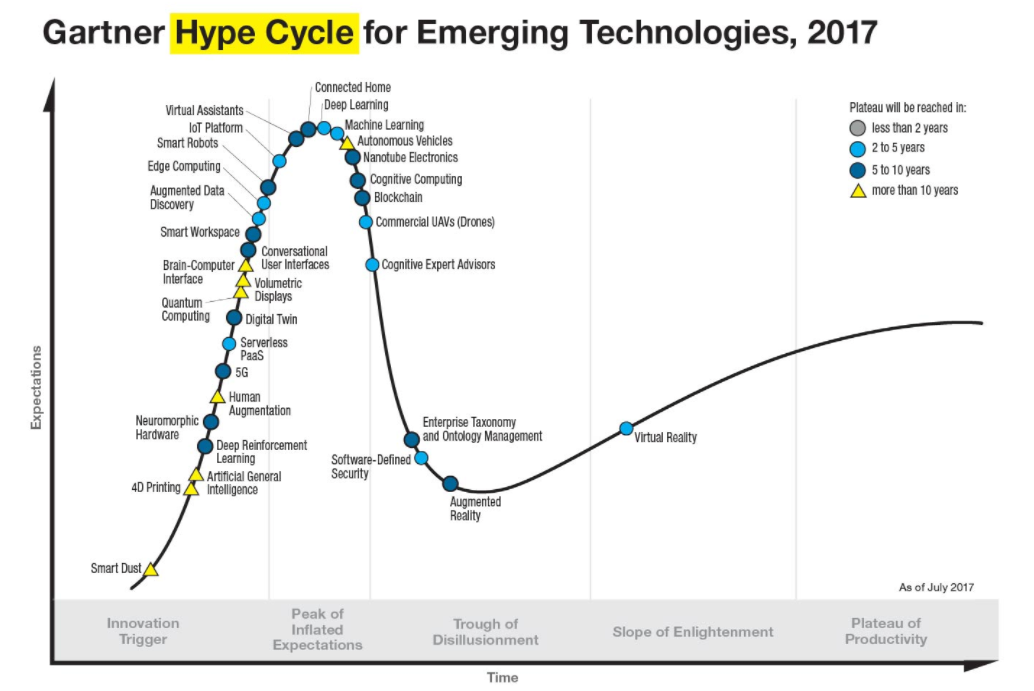
\includegraphics[width=0.8\textwidth]{Images/Gartner.PNG}\\
    \caption{Gartners Hype Cycle 2017}
    \label{fig:Gartner}
\end{minipage}
\\


\subsection{Problem description}
New challenges has emerged as the development of IoT continues to grow, according to \cite{frank} some of them are:

\begin{enumerate}
    \item The scale in terms of units
    \item The constraints in terms of resources: energy, memory, computation
    \item The non-stationary and heterogeneous environments of things.
    
\end{enumerate}

This project will attempt to solve some of the energy constraint IoT designers face today. The project shall explain and build a model of the energy usage of an IoT device which uses GPS. The model shall be so complex that an IoT application can predict the energy cost of getting a positional fix and determine if a method of getting the positional fix is a better substitute. The analyses of the energy usage should also highlight which parameters that are important to include in the energy model. %%%DEVLEOP THIS
\\
\subsection{Motivation}
\cite{frank} also mentions the opportunities in IoT: 
\begin{enumerate}
    \item Many applications only need to provide an overall picture of a situation.
    \item Nodes can	do energy harvesting and the cloud can support nodes with computation.
    \item There	is much data to learn from.
    
\end{enumerate}
This project is part of a ongoing research project at the Faculty of Information Technology and Electronics at NTNU. The research project is called Autonomous Resource-Constrained Things(ART). The aim of the research project is to develop a method for AI to optimize the IoT infrastructure. The first step in developing this method is to analyze and model the energy consumption of the IoT devices. As part of the ART project Ameen Hussain has proposed and evaluated an energy consumption estimation approach for periodic sensing applications running on the IoT devices
devices\cite{Amen}.As the position of an object is one of the most requested information for IoT applications, the usage of GPS has grown substantially.The GPS is used in embedded systems such as watches, trackers, cellphones and cars. GPS can be one of the most power hungry devices in an IoT system. The power budget for an IoT device is often limited, it is therefore useful to have an energy model of the GPS.\\

The student's motivation for choosing this project was to have some insight and experience regarding the different technologies in IoT. The student thinks the experience will be beneficial later as IoT becomes a dominating trend in the Industry. Another motivation was that the Internet of Things combines multiple fields of technology, and challenges the student to apply all of its knowledge of IT and Electronics.
\newpage

\subsection{Methodology}
WRITE THIS LATER
\subsection{Report Structure}

WRITE THIS LATER 
%%%%%%%%%%%%How does a GPS work and draw the state diagram for the GPS.Describe the different alternatives for measuring power consumption of a GPS%%%%%%%%%%%%%%%%%%%%%%%%%





\section{GPS}
The Global positioning system(GPS) is a space based radio navigation system developed by the Unites States Government, and has been operational since 1995.The system provides both timing and geolocation information to a GPS receiver anywhere on the Earth.  The system is not influenced by the number of receivers and can therefore serve an unlimited amount of users. The GPS system can deliver a position which is accurate within 22 meters horizontally if only one receiver is used. If multiple receivers is used positioning accuracy level of the order of a sub-centimeter to a few meters can be obtained \cite{GPS}. 

\subsection{Overview}
GPS consists three segments: space segment, control segment and the user segment. The space segment is a constellation of 24 satellites that are arranged so that  four to ten satellites is visible anywhere on the earth. Each satellite continuously broadcasts a signal composed of two carriers, two digital codes and a navigation message which contains the coordinates of the satellites as a function of the time. Each space vehicle as atomic clocks to ensure the integrity of the navigation message. The codes and the navigation message gets modulated with the two carrier frequencies.  \\If the distance between three satellites are known, the location of the receiver can be determined by measuring the angles with the respect of the each satellite.  GPS needs an additional satellite to account for the clock offset. Figure \ref{fig:GPS} shows the resection that is used by the satellites to determine the position.\\

\begin{minipage}[t]{0.8\textwidth}
\centering
    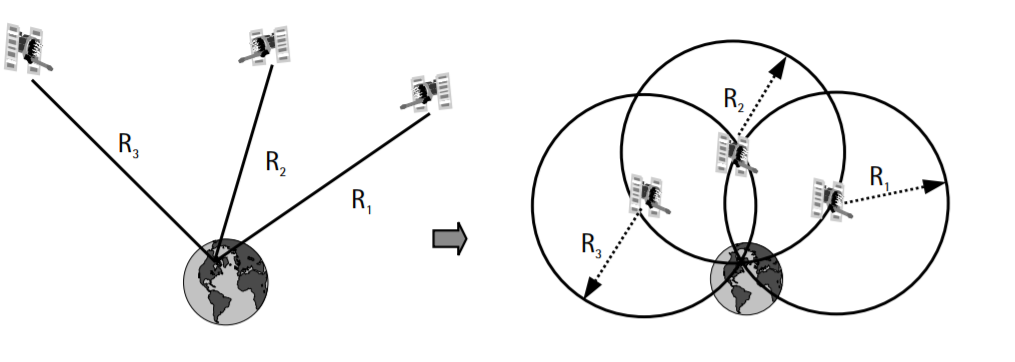
\includegraphics[width=0.8\textwidth]{Images/gps.PNG}\\
    \captionsetup{justification=centering}
    \captionof{figure}{Resection used by the satellites to determine the position}
    \label{fig:GPS}
\end{minipage}


 The distance between the satellite and the receiver are needed for using the method of resection.The Pseudorange is used for measuring the distance by assuming that the clock of the receiver and satellite are synchronized. It is called for pseudorange since they are actually not perfectly synchronized. The receiver can produce the digital codes at the same time instant that the satellites transmits them from space.The distance can be calculated by measuring the difference in delay of the transmitted signal from the produced one. The clocks is actually not perfectly synchronized and this is reason for the name pseudorange. \\
 A method for determining the velocity of a receiver is by estimating the Doppler frequency of the received signal. The Doppler shift is caused by the relative motion of the receiver and the SV. The two carrier frequencies L1 and L2 that the satellites transmits are generated at 1.5 MHz and 1,2 MHz respectively.  Each SV transmits the L1 and L2 signal but the code modulation for each is different to avoid interference. The two digital code coarse acquisition code (C/A) and precision code(P) consists of a stream of binary digits. The codes are generated using an algorithm and enables a receiver to distinguish the satellites since each have their own set of codes. The navigation message contains the ephemeris, the almanac, the health of the SV, the clock correction, and the atmospheric data.The Ephemeris is the precise information about the orbital position and clock correction for the specific satelite. The Alamanac is a coarse orbital data of all the satellites in constellation. The Ephemeris is only valid for four hours and is sent every 30  second, while the Almanac is valid for 180 days and is sent every 12.5 minutes. \\
 The control segment of the GPS system consists of a number of world wide positioned tracking station and a master control station located in the United States. The control segment tracks the satellites to predict their location, control the atomic clock and satellite data that is transmitted by the SV. \\ The user segment is all GPS receivers that is used to determine their position.
  
  
  \subsection{Acquisition and Tracking}
  
  The state diagram of a GPS receiver consists of two distinct states, the acquisition and tracking states shown in figure \ref{fig:GPS reciever}. The acquisition state is the first state that the receiver goes to after start up. This is the state where the receiver searches and tries to detect the C/A codes from the satellites. After detecting and receiving satellite data from minimum four satellites the receiver goes to the tracking state.
 \begin{figure}[H]
\centering
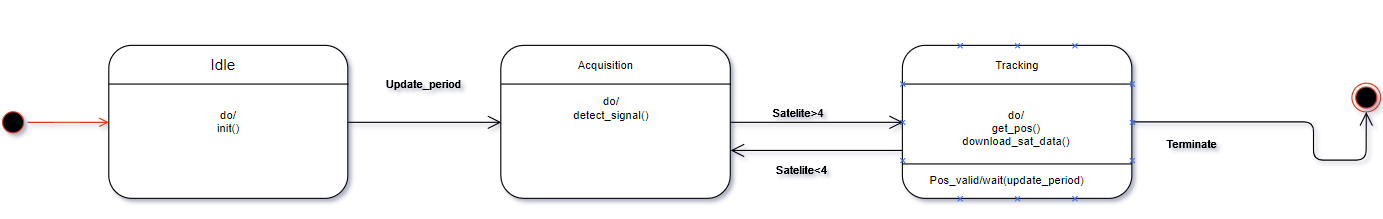
\includegraphics[width=16 cm]{Project_Report/Images/gps_basics.PNG}
\caption{The state diagram of a GPS reciever}
\label{fig:GPS reciever}
\end{figure}

After synchronizing the clock, the receiver determines the position and continues to search for other satellites signals. The receiver goes back to acquisition state if it doesn't detect minimum four strong satellite signals.
Most receivers uses two separate engines for acquisition and tracking, the acquisition is usually the more power hungry of the two states.The time the receiver spends in acquisition state depends on three scenarios:
\begin{itemize}
\item Cold start: This is the same as a factory reset. The receiver doesn't have the last positional fix, the time or any satellite data of the constellation. Standard time to first fix(TTFF) is about 1 minute.
\item Warm start: Last position,time and the Almanac is valid. The receiver does only have to download the Ephirems from the satellites. Standard estimation of TTFF is around 35s.
\item Hot start: When the previous fix was about one second ago, all the data is valid and the estimated time to next fix is 1 second. 

\end{itemize}


\newpage
%%%%Measurment methods for measuring/estimating energy consumption
\chapter{Measurement methods}
As the complexity and energy demand of today's electronics is developing rapidly it's  important to have a good model of the energy usage of in todays industry. Low-power design is therefore one of the biggest research topics in toady's electronics and has produces numerous methods for measuring or estimating the energy consumption of a device. There are several alternatives for modeling the energy consumption of a system where the main difference is that the energy either gets estimated or measured. The following section will present some of these methods. The quality of the estimation and measurement techniques varies from a 20\% error rate to as low as 0.1\%.  The energy consumption can either be estimated before the execution of the program as in software estimation, or it can be directly measured as with a shunt resistor. The appropriate method to use depends on the system that is under measurement, as some of the methods require detailed knowledge of the system, while other threat the system as a black box.
\section{Shunt resistor}
A shunt resistor is often used to measure the energy consumption of a load because of its cost friendly and simple configuration \cite{Intersil} \cite{Infineon} \cite{Vishay}. The shunt is placed in series with the device and the power supply.

If the voltage drop $V_{shunt}$ is measured, the current I can be calculated by Ohms law:\begin{equation}
V_{shunt}=R_{shunt}*I
\end{equation}

$R_{shunt}$ should be of a small value so it doesn't interference with the circuit. The power used by the device can then be calculated by using the power relation \begin{equation}
P=V_{load}*I \\
\end{equation}
\begin{equation}
V_{load}= V_{supply}-V_{shunt}
\end{equation}
\newline The resistor value of the shunt should be of a small value to minimize the power dissipated by the shunt. In \cite{Intersil} it is explained how the resistance value, temperature coefficient and the temperature resistance of the shunt resistor will affect the accuracy of the measurement:
\begin{equation}
\Delta R= R_{initial}* \Delta T * T_{coefficient}\\
\label{rchange}
\end{equation}
\begin{equation}
 \Delta T = \theta * I^{2}*R_{sense}
\end{equation}

The temperature change in the shunt comes mainly from the heat of the power dissipation that is caused by the current flowing into it. A smaller package has a higher thermal resistance $\theta$ and therefore a higher resistance change when power dissipation increases. Figure \ref{fig:Powererror} from \cite{Intersil} shows the error of three different shunt resistors with different packages. 

\begin{minipage}[t]{0.8\textwidth}
\centering
    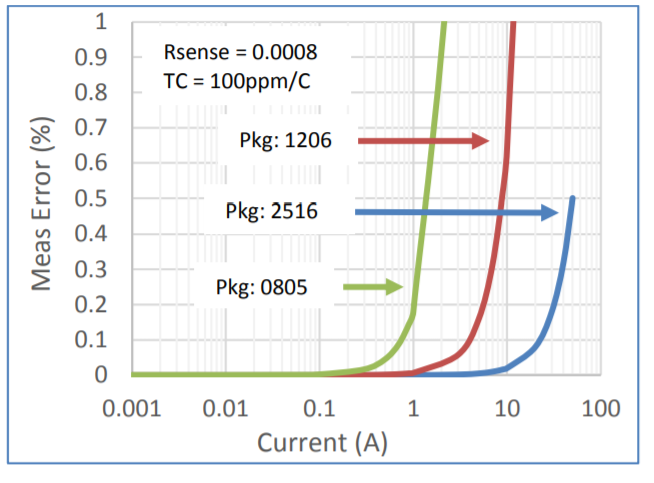
\includegraphics[width=0.8\textwidth]{Images/Powererror.PNG}\\
    \captionsetup{justification=centering}
    \captionof{figure}{The measurement error of three shunt resistors with different packages from \cite{Intersil}}
    \label{fig:Powererror}
\end{minipage}


The shunt can be placed either in a high side or low side configuration. A low-side shunt has one of its terminals grounded, this configuration might be preferable as the shunt resistor is not exposed of the high common node voltage that might had damage the measurement device. The configuration does also give the measurement device an easy access to common ground so that more signals can be measured at the same time in reference to a stable ground.A high-side configuration places the shunt between the power supply and the load. This might be preferable because it connects the load directly to the ground of the power supply. This configuration enables the shunt to detect leakages that appear before the load, which may have not been detected by the low-side configuration. Figure \ref{fig:shunt} shows the two configurations. \hfill \break


\begin{figure}[h]
\centering
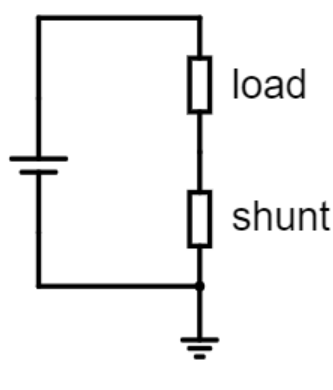
\includegraphics[height=4.5cm]{Project_Report/Images/shunt.PNG}
\caption{The setup for a low-side shunt and a high-side shunt to left and right respectively}
\label{fig:shunt}
\end{figure}




\section{Hall effect}
The Hall effect can be exploited to measure the current in the circuit. When a current $I$ flows in to a conductor it also changes the magnitude of the magnetic field $H$ proportionately. The relation between the flux density $B$ and $I$ can be expressed as follows:


\begin{equation}
B= \mu_{0}*\mu_{r}*H= \frac{\mu{0}*\mu{r}*I}{2\pi r}
\end{equation}

An Hall effect IC consists of a Hall effect sensor which deliver an output signal which is a linear function with the flux density. The IC is a a loss less system because no resistance is inserted into the circuit and therefore a good method of sensing current without interfering the load.  The IC does also require a field concentrator to boost the flux density for the measurement.
\begin{figure}[ht]
\centering
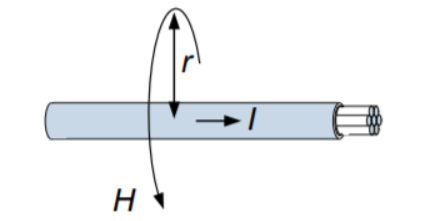
\includegraphics[height=4.5cm]{Project_Report/Images/current.PNG}
\caption{The induced magnetic field of a conductor from \cite{Infineon}}
\label{fig:current}
\end{figure}


\section{Software based estimation}

In \cite{EAC} Kadayif et al presents a framework that can estimate and optimize energy consumption of a high level code. The model is validated by using a cycle-accurate architectural-level energy simulator and is within a 6\% error margin.The input to the framework is its program code, architectural, transistor technology, energy model and the energy constraints.The paper uses a five staged pipeline datapath for the architectural parameter with a 0.35 micro transistor technology. The energy model that the framework uses is the sum of the energy consumed in different components. The components that are used to estimate the energy consumption consist of datapath, bus, main memory, cache and a clock network. Figure \ref{fig:EAC_table} shows the energy-dependent parameters of each component in the energy model and how they can be extracted from the high level code. The energy constraints are only used if optimization of the code is desired. 
\begin{figure}[H]
\centering
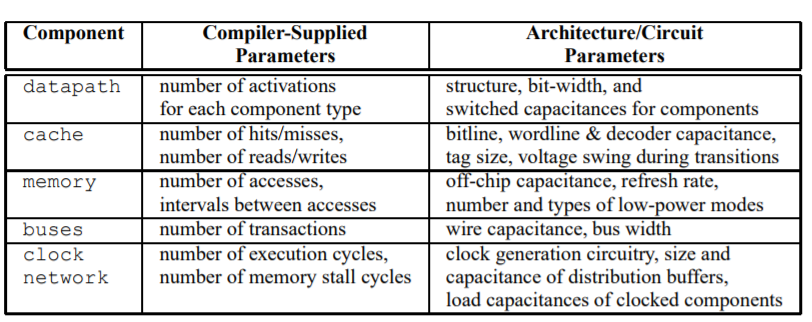
\includegraphics[height=4.5cm]{Project_Report/Images/EAC_table.PNG}
\caption{The energy dependent parameter of each component in the energy model and the belonging parameters in high-level code \cite{EAC}}
\label{fig:EAC_table}
\end{figure}
In \cite{Software_Energy} Deguang et al presents a method for estimating the energy consumption at architecture-level by using an extreme learning machine(ELM).  They model the architecture of the software system as a complex network, where the nodes are the software and the edges between them are the interactions. The energy model they proposed is given by \ref{software equation}

\begin{equation}
 E_{s}= P*T_{s} = f(m_{s})*T_{s}=f(V,E,L,K,C)*T_{s}
\label{software equation}
\end{equation}

$E_{s}$ is the total energy consumption over a $T_(s)$ period. P is the power consumption. $m_{s}$ is the network characteristics and f is the relation between the energy consumption and the network. f depends on the number of nodes V, the number of edges E, average path length L, the clustering coefficient L and the average degree of software network K. By using reverse software engineering they train the ELM to fit the nonlinear correlation function f and uses the ELM to estimate the energy consumption. They compare their model to a pTop model and achieves a 7.9\% error rate. 

\section{Cycle based energy estimation}
 Energy estimation can be done at RTL level by using cycle based energy models. In \cite{Energy_Gupta} Subdoh et al present a macro modeling technique for estimating the energy per cycle for a logic circuit for every input pair vector pair. The paper presents a automatically characterization procedure that can be used to build equation based energy per cycle macro models. The average error of the estimating the energy per cycle is under 20\%. \newline
 
 \cite{Energy_Ana} provides an approach for cycle-accurate hardware/software co-simulations of energy consumption. The simulation framework gets energy estimations for high level descriptions of embedded systems. The energy estimation is obtained by creating energy models for every hardware block and including them in functional models of the "Tool for system simulation"(TSS) simulator. An approach for creating energy models where no structural gate information is known is  presented in the article. 
 
\chapter{Measuring platform}

The method of shunt resistor was chosen to measure the energy consumption of the GPS system. The shunt resistor was chosen due to its low complexity compared to the Hall effect IC.  The other software estimation techniques and cycle aware techniques was not chosen, as they either tries to estimate the energy consumption with poor accuracy or they need non available RTL information about the design. The shunt resistor threats the system that is getting measured as a black box, which enables the measuring platform to be used with any system. Two configurations of the measurement platform with a shunt resistor was developed. This section will explain the functionality of each component of the measurement platfrom.


\section{PicoScope 640 AD}
PicoScope 6000 from Picotecnology is a 4 channel digital oscilloscope with 5GS/s sampling and 2 GSample buffer memory \cite{Pico}. The oscilloscope is equipped with USB 3.0 and supplied with an SDK that enables the user to write their own software. The PicoScope has advanced trigger possibilities and a bandwidth of 500MHz along with a signal generator. The oscilloscope is used to measure the voltage drop across the shunt resistor.   

\section{PC with python script}
A Python API that uses the SDK from Picoscope is executed on the PC. The script is a modified version of the framework by Amen Hussain \cite{Amen}. The script is included in the appendix \ref{Appendix:EnergyMeasure.py}. The script measures the voltage drop over the shunt resistor by using the following parameters:

\begin{itemize}
    \item sampling- The sampling frequency 
    \item duration- The length of each waveform
    
\end{itemize}
The sampling and duration is used to generate a waveform of the sampled data.
The sequence diagram in figure \ref{fig:sequence} shows the interaction between the python script and the oscilloscope.  

\begin{figure}[H]
\centering
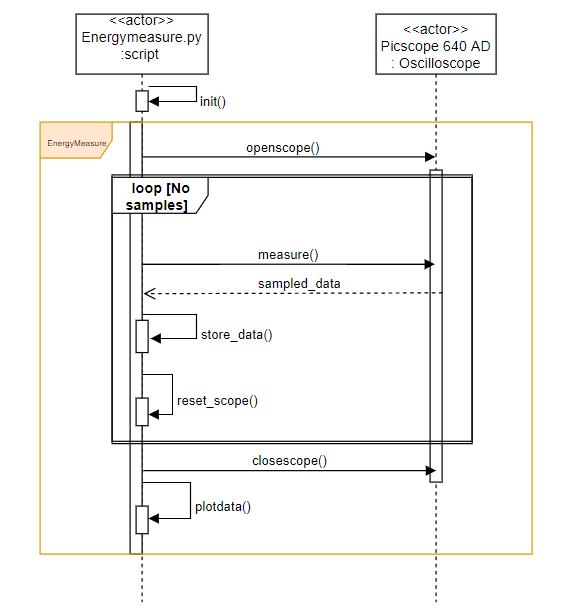
\includegraphics[height=10.5cm]{Project_Report/Images/Sequence_diagram.PNG}
\caption{Sequence diagram for the measurement script}
\label{fig:sequence}
\end{figure}
 

 The script samples the data and stores it in a list, before it restarts the sampling for the next waveform. An overhead of storing data and initializing the oscilloscope before each sample introduces a limit for the processing speed of the measurements. The measured delay caused by the overhead in software is 20-50 milliseconds between each waveform. The delay is found by using timers in software during the execution of the python script. This means that some data is not captured during the overhead process and constrains the accuracy of the measurements.
The Python script generates a plot of each waveform after the data has been analyzed \ref{fig:pythonwaveform}

\begin{figure}[H]
\centering
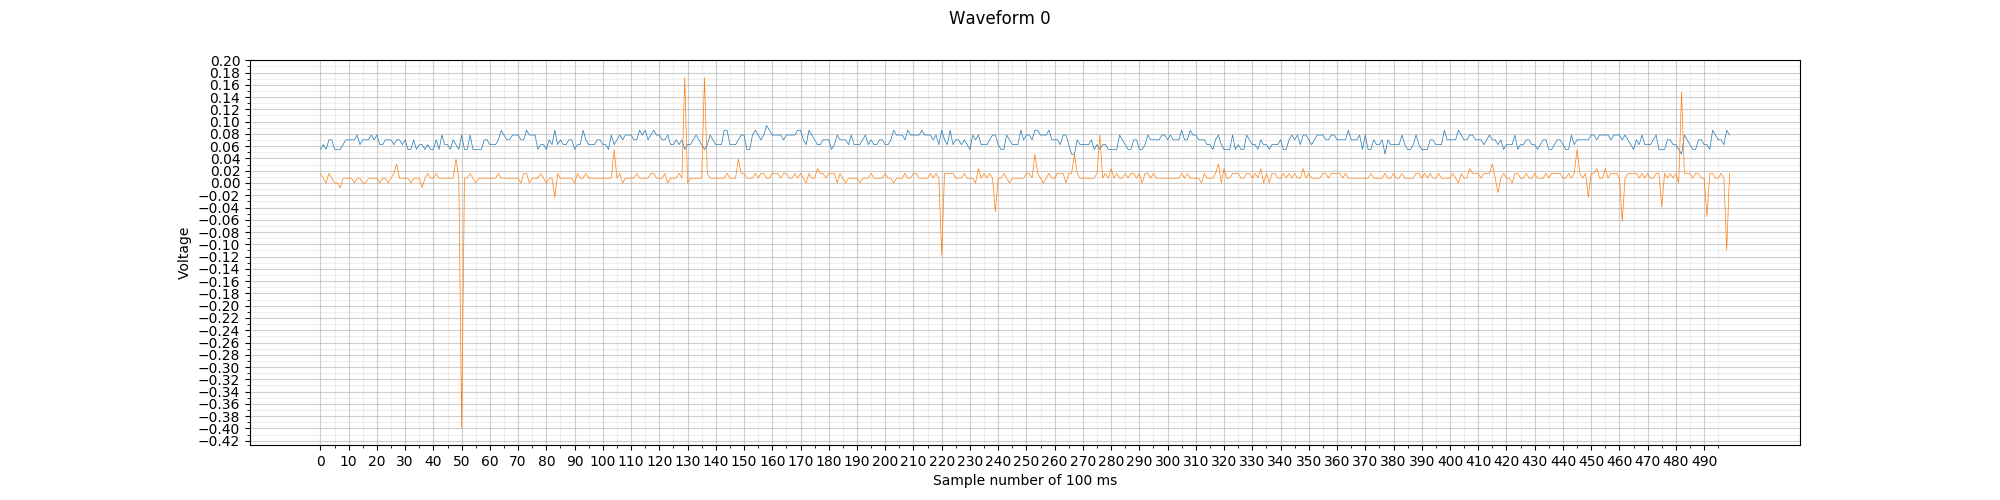
\includegraphics[height=4.5cm]{Project_Report/Images/pythonwaveform.png}
\caption{The waveform that is plotted by the python script and used for analyzing the current consumption}
\label{fig:pythonwaveform}
\end{figure}
 
An Excel document with the average current and power of each waveform is also generated. Figure \ref{fig:waveexcel} shows a screenshot of the generated excel spreadsheet for 13 waveforms.

\begin{figure}[H]
\centering
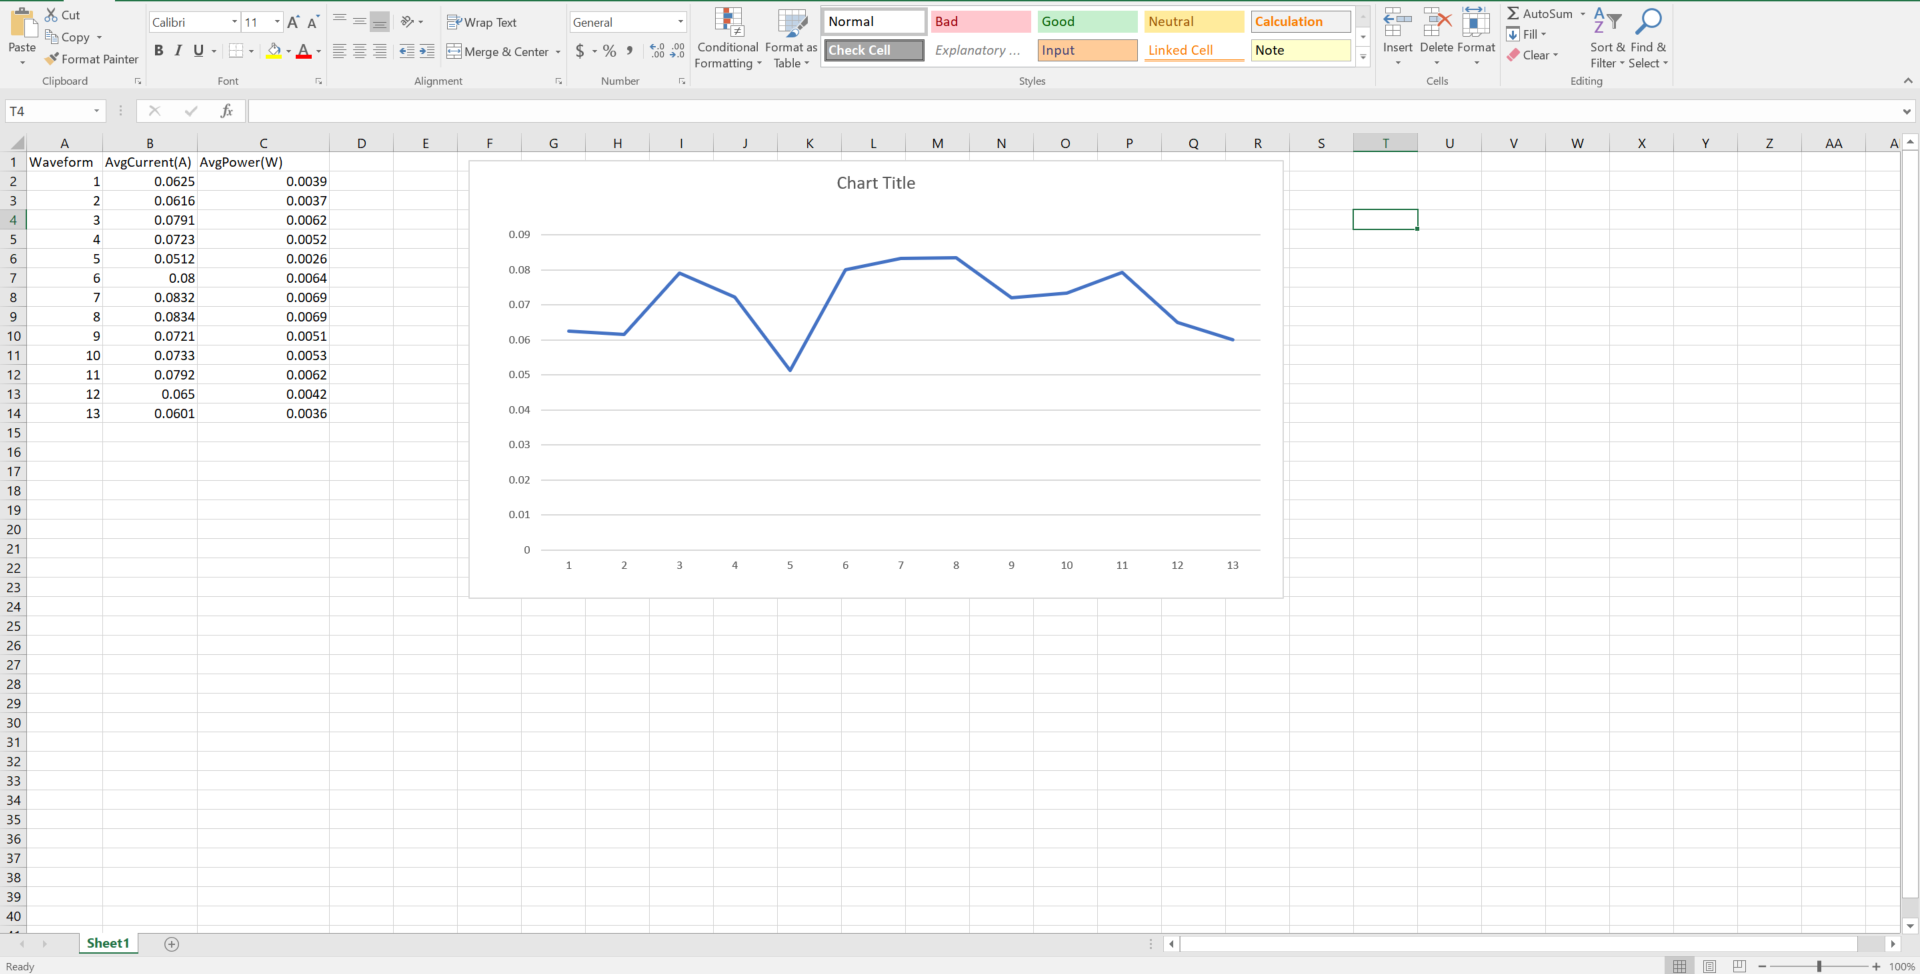
\includegraphics[height=8.0cm]{Project_Report/Images/waveformexcel.PNG}
\caption{Spreedsheet with the average current of 13 waveforms}
\label{fig:waveexcel}
\end{figure}
 



\section{Configuration options}
 Two configurations of the measurement platform with shunt resistor was developed. The first used a C027 application board from u-blox, while the other used a LoPy microcontroller from PyCom. Both methods used the PC and the Oscilloscope. 
 


\subsection{Configuration with C027}
Figure \ref{fig:deploy_C027} shows the deployment diagram of the configuration with the C027 development kit.  

\begin{figure}[H]
\centering
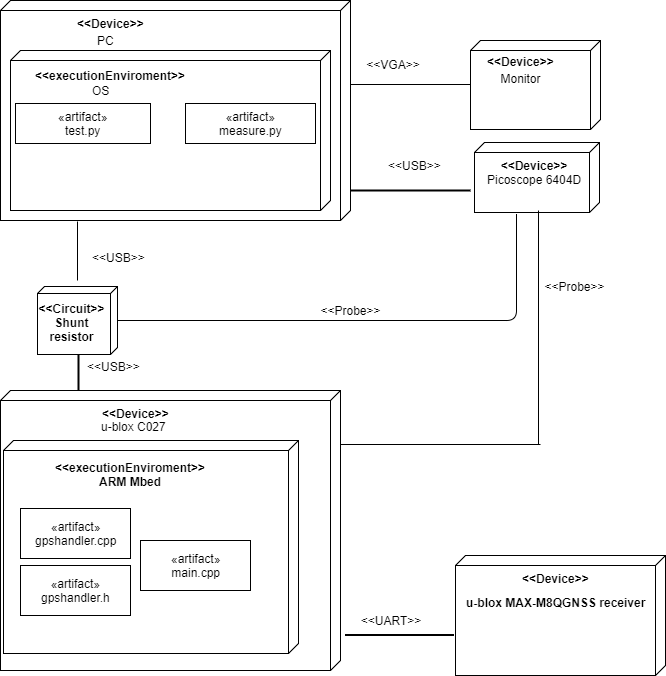
\includegraphics[height=9.5cm]{Project_Report/Images/C027_deploy.png}
\caption{Deployment diagram of the configuration with the C027}
\label{fig:deploy_C027}
\end{figure}
\vspace{5mm}The u-blox C027 is a development board for IoT applications that supports GSM, UMTS and CDMA networks. The development board has a MAX-M8Q GNSS receiver and a cellular module. The header connector has 6 analog inputs, 9 PWM, 22 GPIO, 1 SPI, 1 I2C, 1 UART and 1 I2S. C027 is supported by ARM Mbed, which is an operating system for IoT devices \cite{C027}. The application board has no embedded low power mode, but some peripherals like the GPS can be turned off with UART. Time to first fix (TTFF) for the receiver is \cite{MAX-M8}:
\begin{itemize}
    \item Cold start: 30s
    \item Hot  start: 1s
\end{itemize}

Two threads are run in "main.cpp" on the C027, the first thread receives the requested command from the PC and updates a shared variable between the two threads. The value of the shared variable corresponds to a predefined action. The second thread checks the value of the shared variable and executes the action by sending a certain sequence of bits over UART to the GPS. At the same time the action is executed, a GPIO pin is pulled high to signalize to the PC that a measurement should be done. The code that was written for C027 is included in the appendix \ref{Appendix:C027.Cpp}. 

To measure the current consumption of the application board, we had to put the shunt resistor between the VCC and GND from the USB connection. The VCC for the USB connection could not be sinked from the USB port, because the value of the VCC would not be constant 5v and therefore introduce an error to the measurement. We decided therefore to use a 12 V battery and the LM317 voltage regulator for producing the VCC for the application board. Figure \ref{fig:Schematic_C027} shows the schematic of the C027 configuration with the LM317 voltage regulator. 

\begin{figure}[H]
\centering
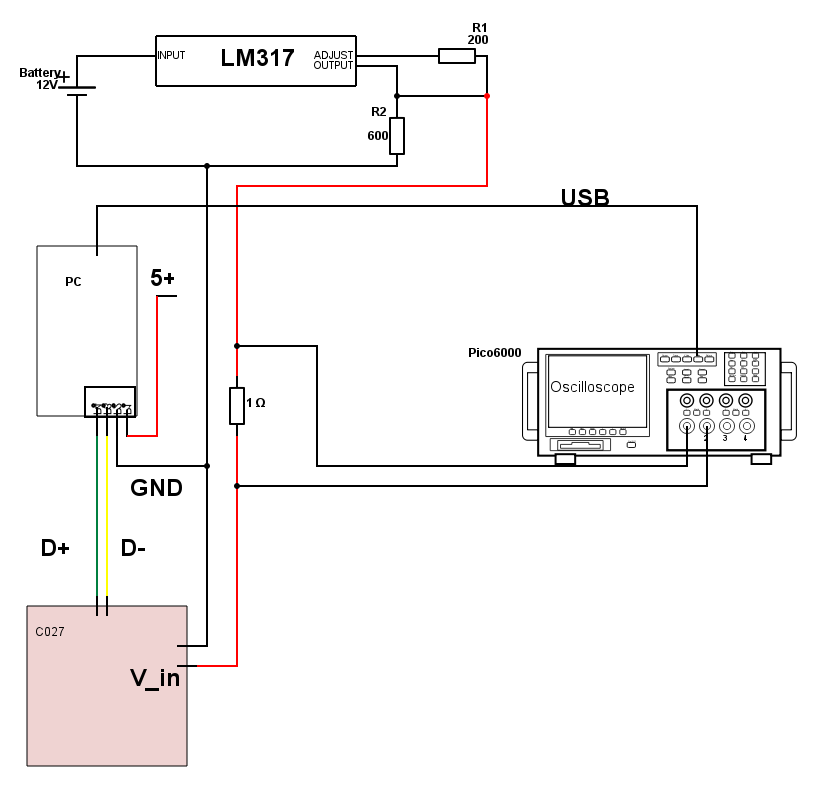
\includegraphics[height=6.5cm]{Project_Report/Images/C027_Schematic.png}
\caption{Schematic of the C027 configuration}
\label{fig:Schematic_C027}
\end{figure}

The oscilloscope measures the voltage after shunt resistor. The voltage drop over the shunt resistor is estimated by first measuring the output of the voltage regulator, and then measuring the voltage after the shunt resistor and subtracting them in software. Measuring the voltage drop directly will change the common ground for the oscilloscope, C027 and the PC to the node after the shunt resistor. This is undesired, because it prevents the oscilloscope from measuring another signal which is not referenced to that GND. 

Difficult debugging, short circuiting of the PC and a too complex configuration encouraged us to develop another simpler measurement platform. 



\subsection{Configuration with LoPy}
Another option for the measurement platform was a circuit with the LoPy microcontroller from Pycom. An overview over the measurement platform is shown in \ref{fig:LoPy_deploy}. 

\begin{figure}[H]
\centering
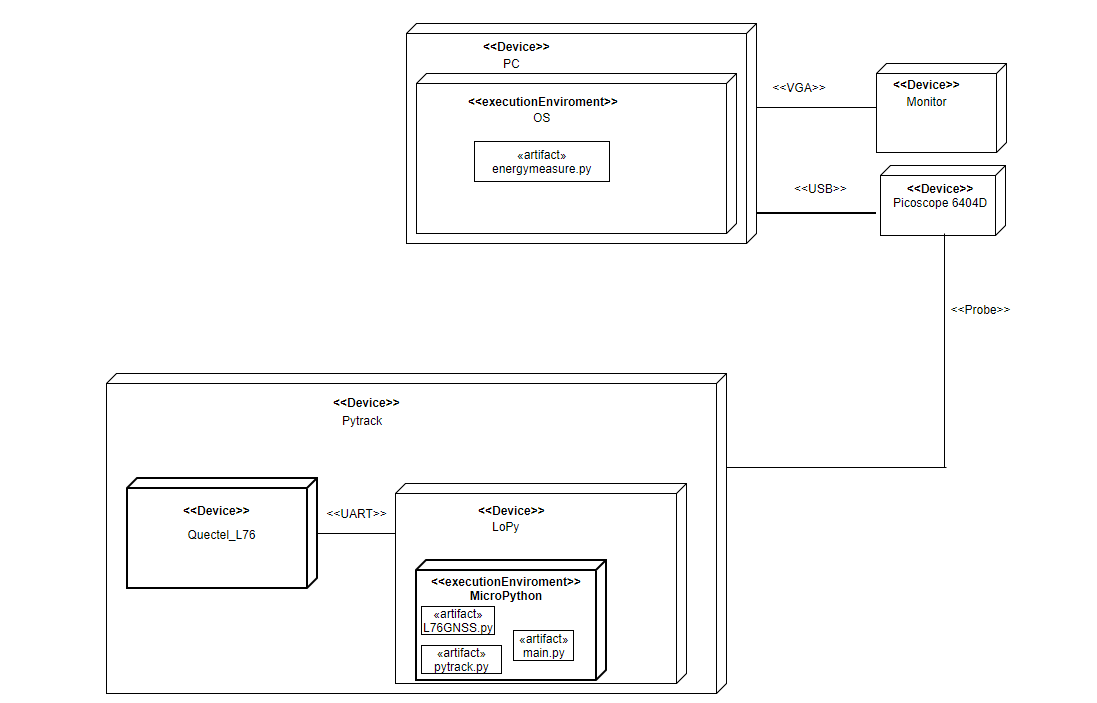
\includegraphics[height=9.5cm]{Project_Report/Images/LoPy_deploy.png}
\caption{Deployment diagram of the LoPy configuration}
\label{fig:LoPy_deploy}
\end{figure}

The LoPy is a microcontroller equipped with a LoRa, Wifi and BLE technology \cite{LoPy} and is specifically made for IoT use cases. It uses the Espressif ESP32 chip and the user write the program code in Micropython. LoPy has a low-power feature which makes it turn off most of the hardware except its internal peripheral. The micro controller has UART, SPI, I2C and up to 24 GPIO.

The LoPy is equipped with Pycom's Pytrack, which is an extension shield to the LoPy. Pytrack is equipped with a L76-l GPS receiver from Quectel and a 3 axis 12 bit accelerometer \cite{Pytrack}. L76-l is a low power GNSS receiver \cite{L76}. The module is equipped with an ARM7 processor and UART for serial communication. The LoPy controls the receiver through the execution of the program code and communicates with the ARM7 processor through serial communication with the Pytrack shield. TTFF for the GNSS receiver is:
\begin{itemize}
\item Cold start:35s
\item Warm start: 30s
\item Hot start: 1s


\end{itemize}


The LoPy offers debugging possibilities over WiFI which enables a simple configuration by measuring the voltage drop directly over the shunt resistor. The schematic of the circuit configuration is shown in \ref{fig:LoPy_Schematic}. The green channel is the common ground for both the red channel and the black channel. The red channel measures the voltage drop over the shunt. The measured signal is inverted in software, because it is referenced to a node that has a higher potential. 

\begin{figure}[H]
\centering
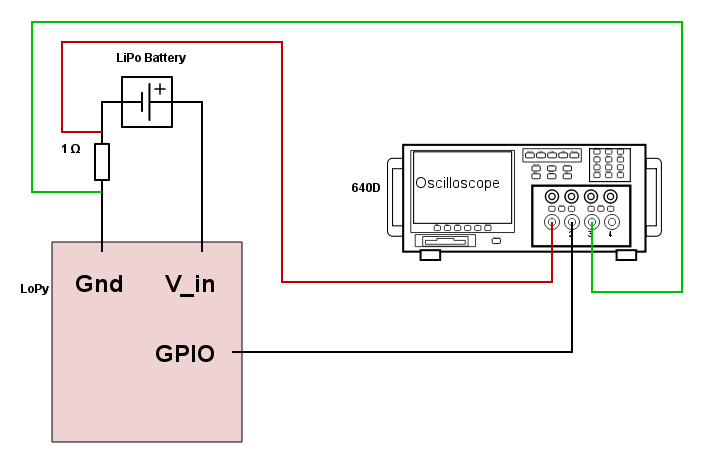
\includegraphics[height=6.5cm]{Project_Report/Images/LoPy_Schematic.png}
\caption{A low side shunt configuration}
\label{fig:LoPy_Schematic}
\end{figure}


\subsubsection{Program code for acquiring a positional fix}
Program code was written for the LoPy. The code was based on the framework published from PyCom. The code initializes the serial communication with the ARM microcontroller on the Quectel L76-l receiver. The next step is to parse the satellite data that is sent from the receiver to the LoPy. The data is sent according to the NMAE protocol. A part of the program code is shown in \ref{code:Parsing of gpsdata}. The code reads the data from serial and tries to find the GPGGA data. The GPGGA contains the fix status and other satellite data. If the GPGGA data is found, the fix status is read and set. The remaining code is included in the appendix \ref{Appendix:L76GNSS.py}

\lstset{language=Python}          % Set your language (you can change the language for each code-block optionally)

\begin{lstlisting}[frame=single]  % Start your code-block

            nmea += self._read().lstrip(b'\n\n')
            .rstrip(b'\n\n')
            gpgga_idx = nmea.find(b'GPGGA')
            if gpgga_idx >= 0:
                gpgga = nmea[gpgga_idx:]
                e_idx = gpgga.find(b'\r\n')
                if e_idx >= 0:
                    try:
                        gpgga = gpgga[:e_idx].decode('ascii')
                        print (gpgga)
                        self.gpgga_s = gpgga.split(',')
                        print(self.gpgga_s)
                        self.get_fix()
                        if(self.fix >0):
                            self.lat_d, self.lon_d
                            = self._convert_coords
                            (self.gpgga_s)
\end{lstlisting}
\label{code:Parsing of gpsdata}









.
\newpage
\chapter{Measurements}

 This chapter presents the results and the program code that was used during the  specific test. 






\section{Current Consumption}

The first step was to measure the current consumption of the LoPy during a request of positional fix. Measuring of data was done outside with the measurement platform. All the measurements was done under similar weather conditions. 


\subsection{Measurement with communication}
Program code for getting a positional fix is shown in \ref{code:intial}. The program initialize a GPIO pin that is toggled when the positional fix is acquired. The function coordinates() is from the l76 GNSS class, and sets the class variable fix when the position is received. 
\lstset{language=Python}          % Set your language (you can change the language for each code-block optionally)
\begin{lstlisting}[frame=single,caption = main.py]  % Start your code-block

#intialize the trigger output and the Pytrack/GPS
p_out = Pin('P20', mode=Pin.OUT)
p_out.value(0)
py = Pytrack()
l76 = L76GNSS(py)
while (True):
    #Toggle the trigger when a fix acquried
    coord = l76.coordinates()
    print ("FIX: ", l76.fix)
    if ((l76.fix) and not(l76.first_fix)):
        l76.first_fix = 1
        l76._set_time()

        p_out.value(1)
        time.sleep(0.25)
        p_out.value(0)
\end{lstlisting}
\label{code:intial}
After doing some measurements with the program code and analyzing it, it became evident that another power demanding task was running on the LoPy besides the GPS function. The current and power consumption of the 5 first waveforms are shown in table \ref{Table:WIFI_ON}.
\begin{table}[h!]
\begin{center}
 \begin{tabular}{||c c c||} 
 \hline
 Waveform & Avg Current(A) & Power(W)\\ [0.5ex] 
 \hline\hline
 1 & 0.1433    & 0.0205 \\ 
 \hline
 2 & 0.1421    & 0.02020 \\
 \hline
 3 & 0.1365  & 0.0186 \\
 \hline
 4 & 0.1334  & 0.0178 \\
 \hline
 5 & 0.1399  & 0.01958 \\ 
 \hline
 \rowcolor{red}
 6 & 0.1439    & 0.0207 \\ 
 \hline
 7 & 0.1347  & 0.0181 \\
 \hline
 8 & 0.1358  & 0.01846 \\
 \hline
 9 & 0.1358    & 0.01925 \\[1ex]
 \hline
\end{tabular}
\end{center}
\caption{The 9 waveforms after the initial startup sequence}
\label{Table:WIFI_ON}
\end{table}

The row highlighted in red, is the waveform with the highest average current and power consumption.
Figure \ref{fig:startup_intial} shows the plot of waveform 6 that is made with \ref{fig:sequence}.


 \begin{figure}[H]
\centering
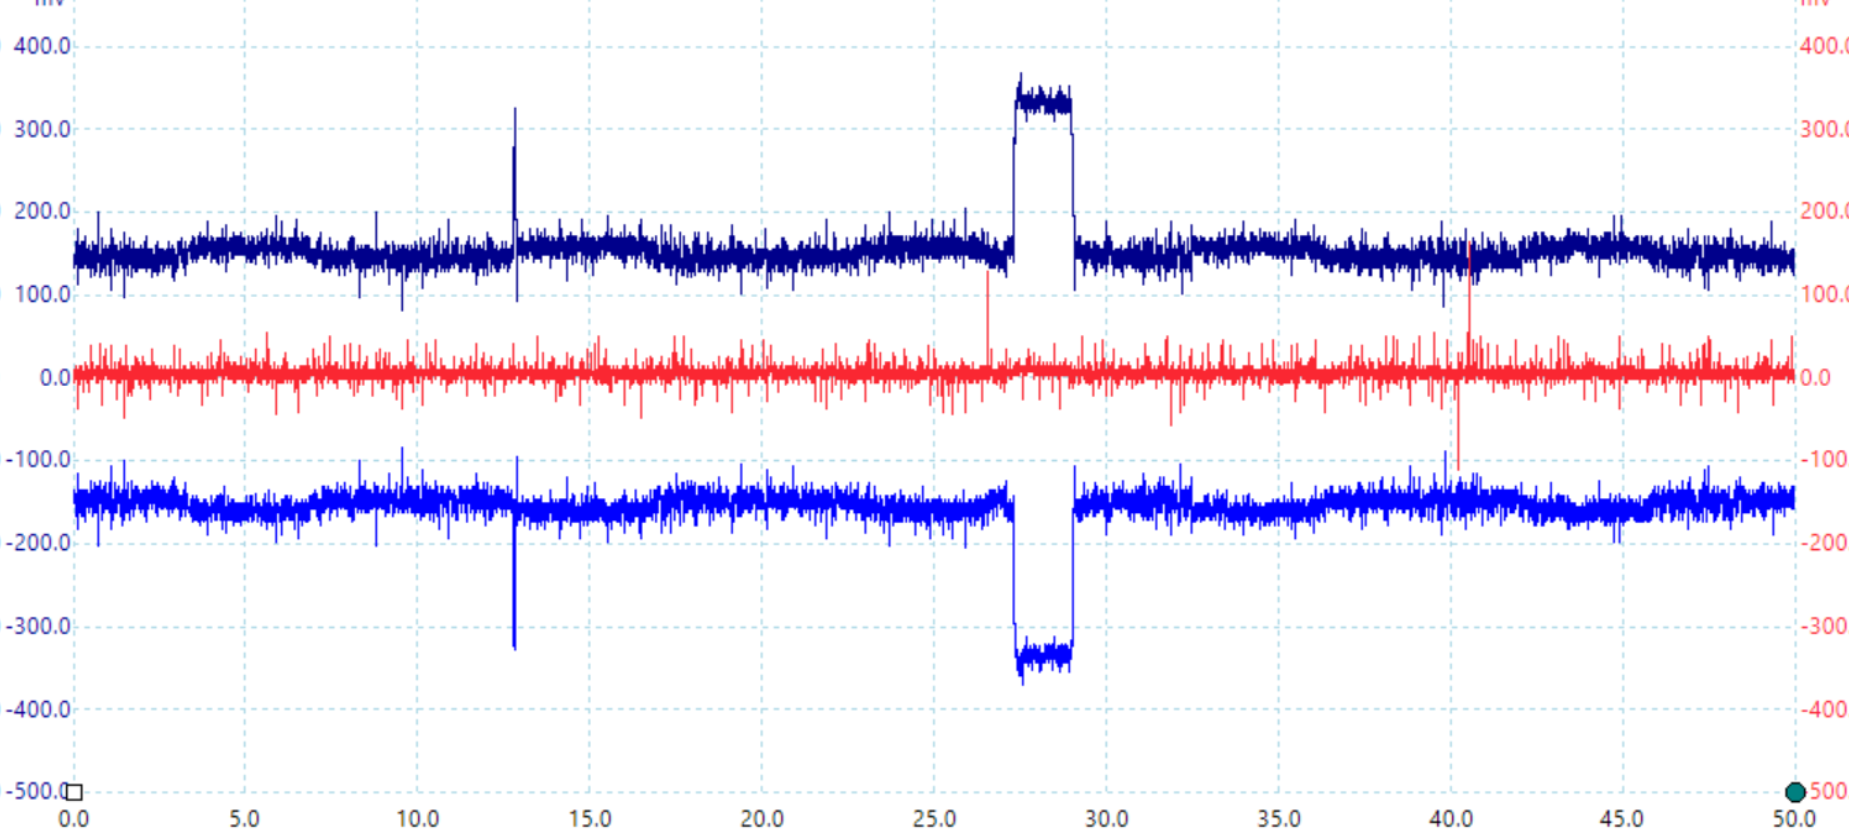
\includegraphics[width=18 cm]{Project_Report/Images/startup_intial.PNG}
\caption{Waveform 6 with the voltage drop(blue) and trigger(orange)}
\label{fig:startup_intial}
\end{figure}

 The conversion from the measured voltage to current is 1:1, since a 1 ohm resistor is used. The signal have an periodic surge around 430 mA. There are 100 samples between each pulse. A sampling frequency of 5000 S/s gives a sampling interval:
 \begin{equation}
     p= \frac{1}{f} = \frac{1}{5000S/s}= 0.0002 s = 0.2 ms 
 \end{equation}
 
 The period of the pulse with a sampling period of 0.2 ms and 100 samples between is:
 
 \begin{equation}
     p_pulse = 100*0.2 ms = 20 ms
 \end{equation}
 After reviewing the results, it becomes obvious that the high average current is due to the disturbance from the periodic signal. The periodic signal makes it difficult to relate the power consumption to the GPS, as it influences the current consumption.


\section{Measurements without communication}

The periodic signal is understood as the communication protocol of the WIFI and Bluetooth. The first part of the improved program code, turns the wireless protocols off to remove the disturbance. A COLD START is sent to the ARM processor to reset the GPS between each execution to remove all satellite data. A deepsleep is included after a fix has been acquired. The LoPy restarts the program code after waking up from deepsleep. Figure \ref{code:wifioff} shows the programcode.

\lstset{language=Python}          % Set your language (you can change the language for each code-block optionally)
\begin{lstlisting}[frame=single, caption= main.py without communication]  % Start your code-block

# initialize ``P9`` in gpio mode and make it an output
p_out = Pin('P20', mode=Pin.OUT)
p_out.value(0)
wlan= WLAN()
wlan.deinit()
bt = Bluetooth()
bt.deinit()

py = Pytrack()
l76 = L76GNSS(py

py.setup_sleep(2)
l76.write_gps(l76.COLD_START,False)
time.sleep(2)

p_out.value(1)
time.sleep(2)
p_out.value(0)

while (True):
    coord = l76.coordinates()
    print ("FIX:jared ", l76.fix)
    if ((l76.fix) and not(l76.first_fix)):
        l76.first_fix = 1
        l76._set_time()

        p_out.value(1)
        time.sleep(0.25)
        p_out.value(0)
        py.go_to_sleep(True):
\end{lstlisting}
\label{code:wifioff}

Figure \ref{fig:WIFI_OFF} shows a screenshot of the generated excel from a test run. The document contains the average current, average power and the value of the trigger signal B for each waveform. The screenshot shows the initializing phase when WIFI and Bluetooth is turned off. 14000 waveforms is sampled during the test run of the program code. A test run lasts for 1 hour.  


\begin{figure}[H]
\centering
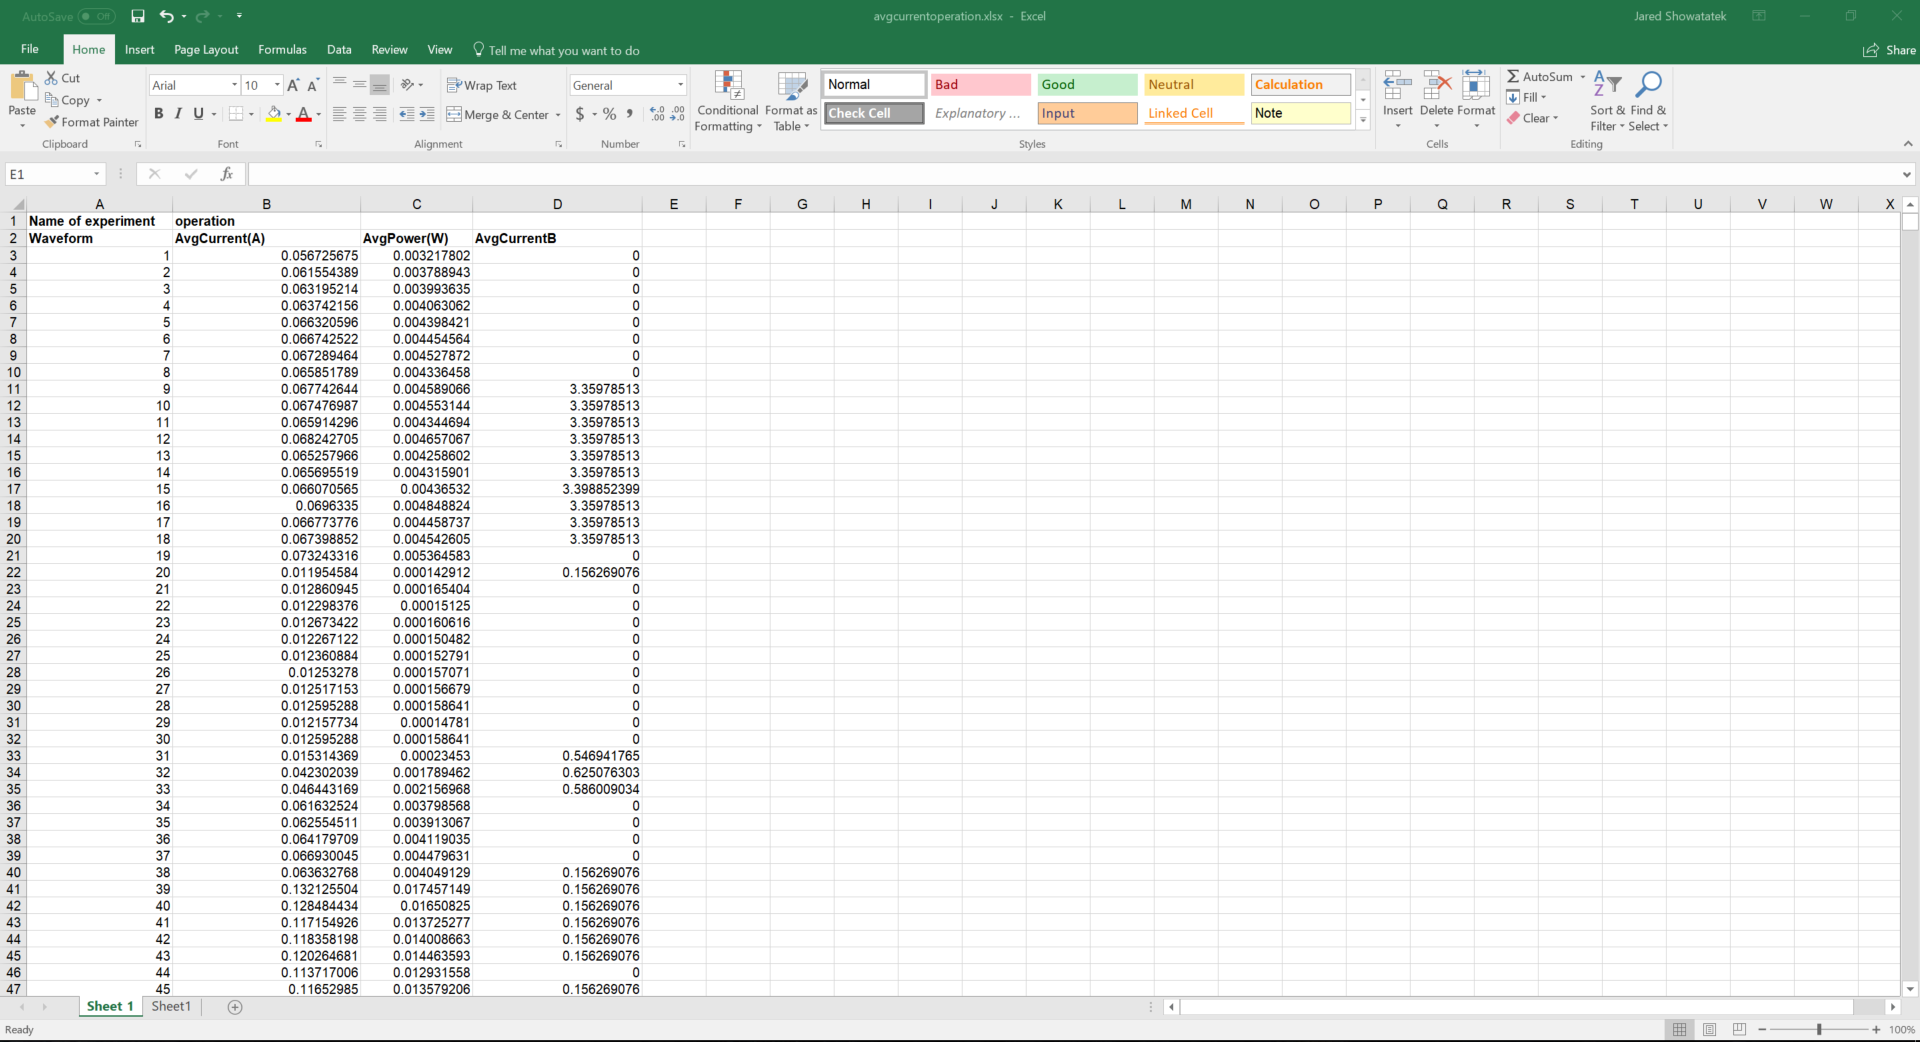
\includegraphics[width=16 cm]{Project_Report/Images/wifioff.PNG}
\caption{The excel document with the data from a test run}
\label{fig:WIFI_OFF}
\end{figure}

Table \ref{Table:wifioff} shows the data when a positional fix is acquired.  
\begin{table}[h!]
\begin{center}
 \begin{tabular}{||c c c c||} 
 \hline
 Waveform & AvgCurrentA(A) & Power(W) & AvgCurrentB(A) \\ [0.5ex] 
 \hline\hline
 4831 & 0.0796 & 0.0063 & 0 \\ 
 \hline
 4832 & 0.0830 & 0.0069 & 0 \\
 \hline
 4833 & 0.0759  & 0.0057 & 3.3 \\[1ex]
 \hline
\end{tabular}
\end{center}
\caption{The data right before}
\label{Table:wifioff}
\end{table}

The plot for waveform 4832 and waveform 4833 is shown in \ref{fig:4832} and \ref{fig:4833}
\begin{figure}[H]
\centering
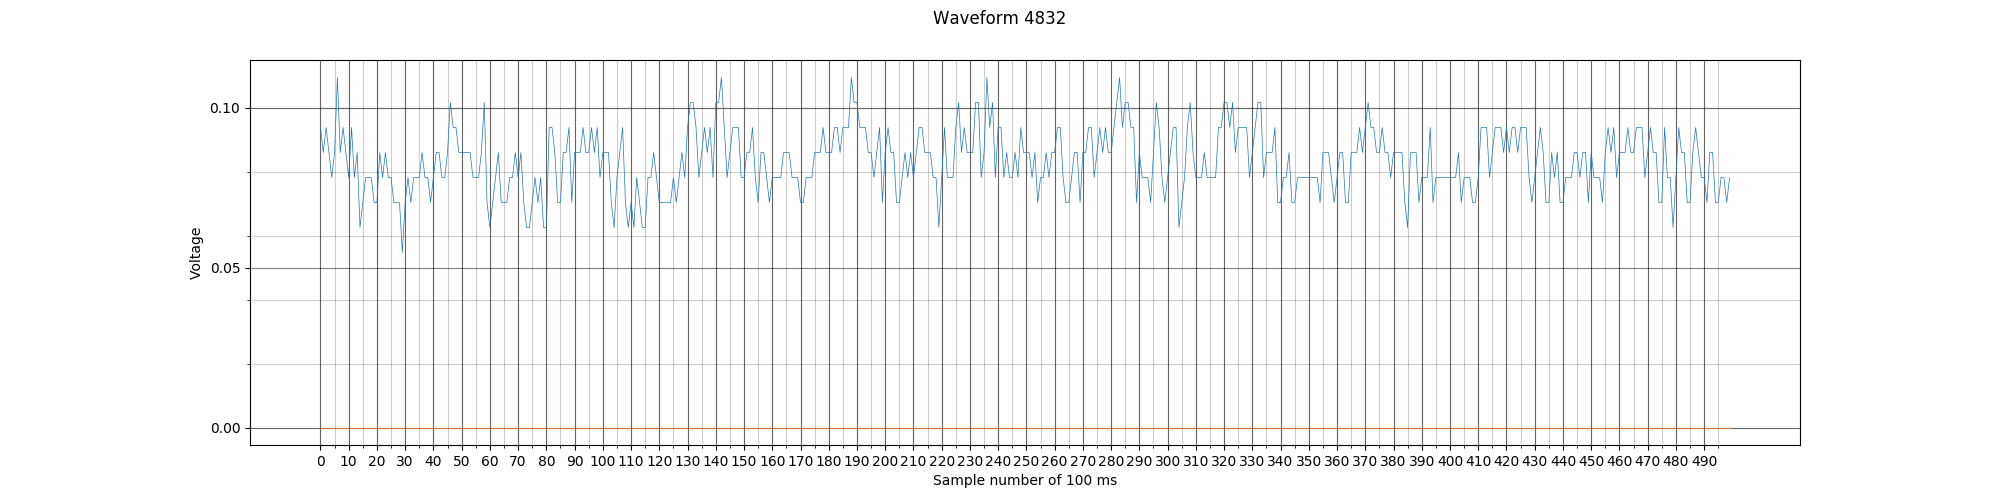
\includegraphics[width=16 cm]{Project_Report/Images/4832.png}
\caption{Waveform 4832 right before a positional fix is acquired)}
\label{fig:4832}
\end{figure}

\begin{figure}[H]
\centering
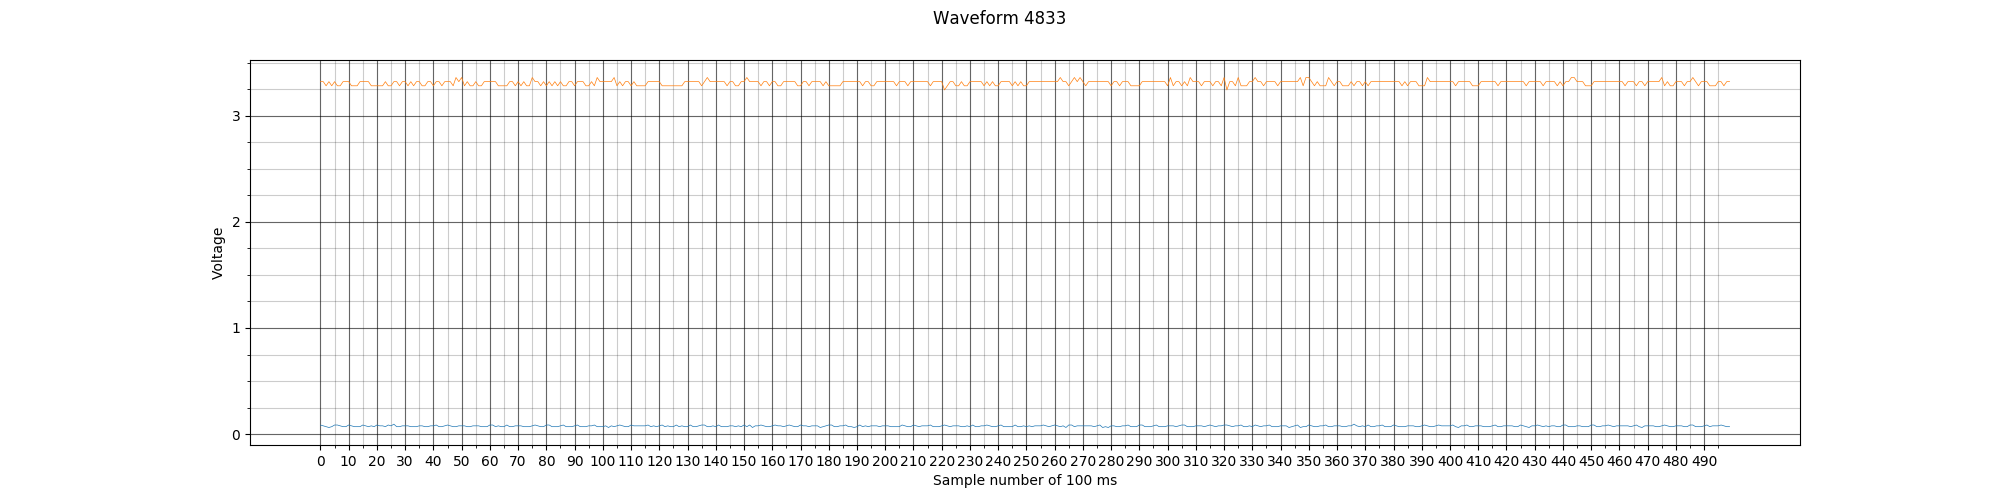
\includegraphics[width=16 cm]{Project_Report/Images/4833.png}
\caption{The waveform when a fix is acquired and the trigger is set}
\label{fig:4833}
\end{figure}




\section{Measuring of deep sleep}
The time from waking up the LoPy from deepsleep until it is searching for signals in the acquisition phase is estimated. The program code used for testing is shown in \ref{code:deepsleep}

\lstset{language=Python}          % Set your language (you can change the language for each code-block optionally)
\begin{lstlisting}[frame=single,caption = main.py for deepsleep measurement]  % Start your code-block

# initialize ``P9`` in gpio mode and make it an output
p_out = Pin('P20', mode=Pin.OUT)
p_out.value(0)

wlan= WLAN()
wlan.deinit()
bt = Bluetooth()
bt.deinit()
py = Pytrack()
l76 = L76GNSS(py)
py.setup_sleep(5)
py.go_to_sleep(True)
l76.write_gps(l76.COLD_START,False)
time.sleep(2)
p_out.value(1)
time.sleep(2)
p_out.value(0)
print("after init")
while (True):
    coord = l76.coordinates()
    print ("FIX:", l76.fix)
    p_out.value(1)
    time.sleep(2)
    p_out.value(0)
    py.go_to_sleep(True)
    if ((l76.fix) and not(l76.first_fix)):
        l76.first_fix = 1
        l76._set_time()

        p_out.value(1)
        time.sleep(0.25)
        p_out.value(0)
\end{lstlisting}
\label{code:deepsleep}


The time is estimated by counting the number of waveforms of 100 ms that is sampled before the initializing sequence signals appears. This time is added together with the overhead of sampling data between each waveform. 42 waveforms is sampled before the initializing sequence appears. 
\begin{equation}
100 ms * 42 = 4.2 s
\end{equation}
\begin{equation}
3.8 s + (20ms*42) = 5.04 s \approx  5 s
\end{equation}

The average current in deep sleep is measured to 3.2 mA. The average current during the initializing sequence is 101 ma. The generated excel document with data is shown in figure \ref{fig:deepsleep}

\begin{figure}[H]
\centering
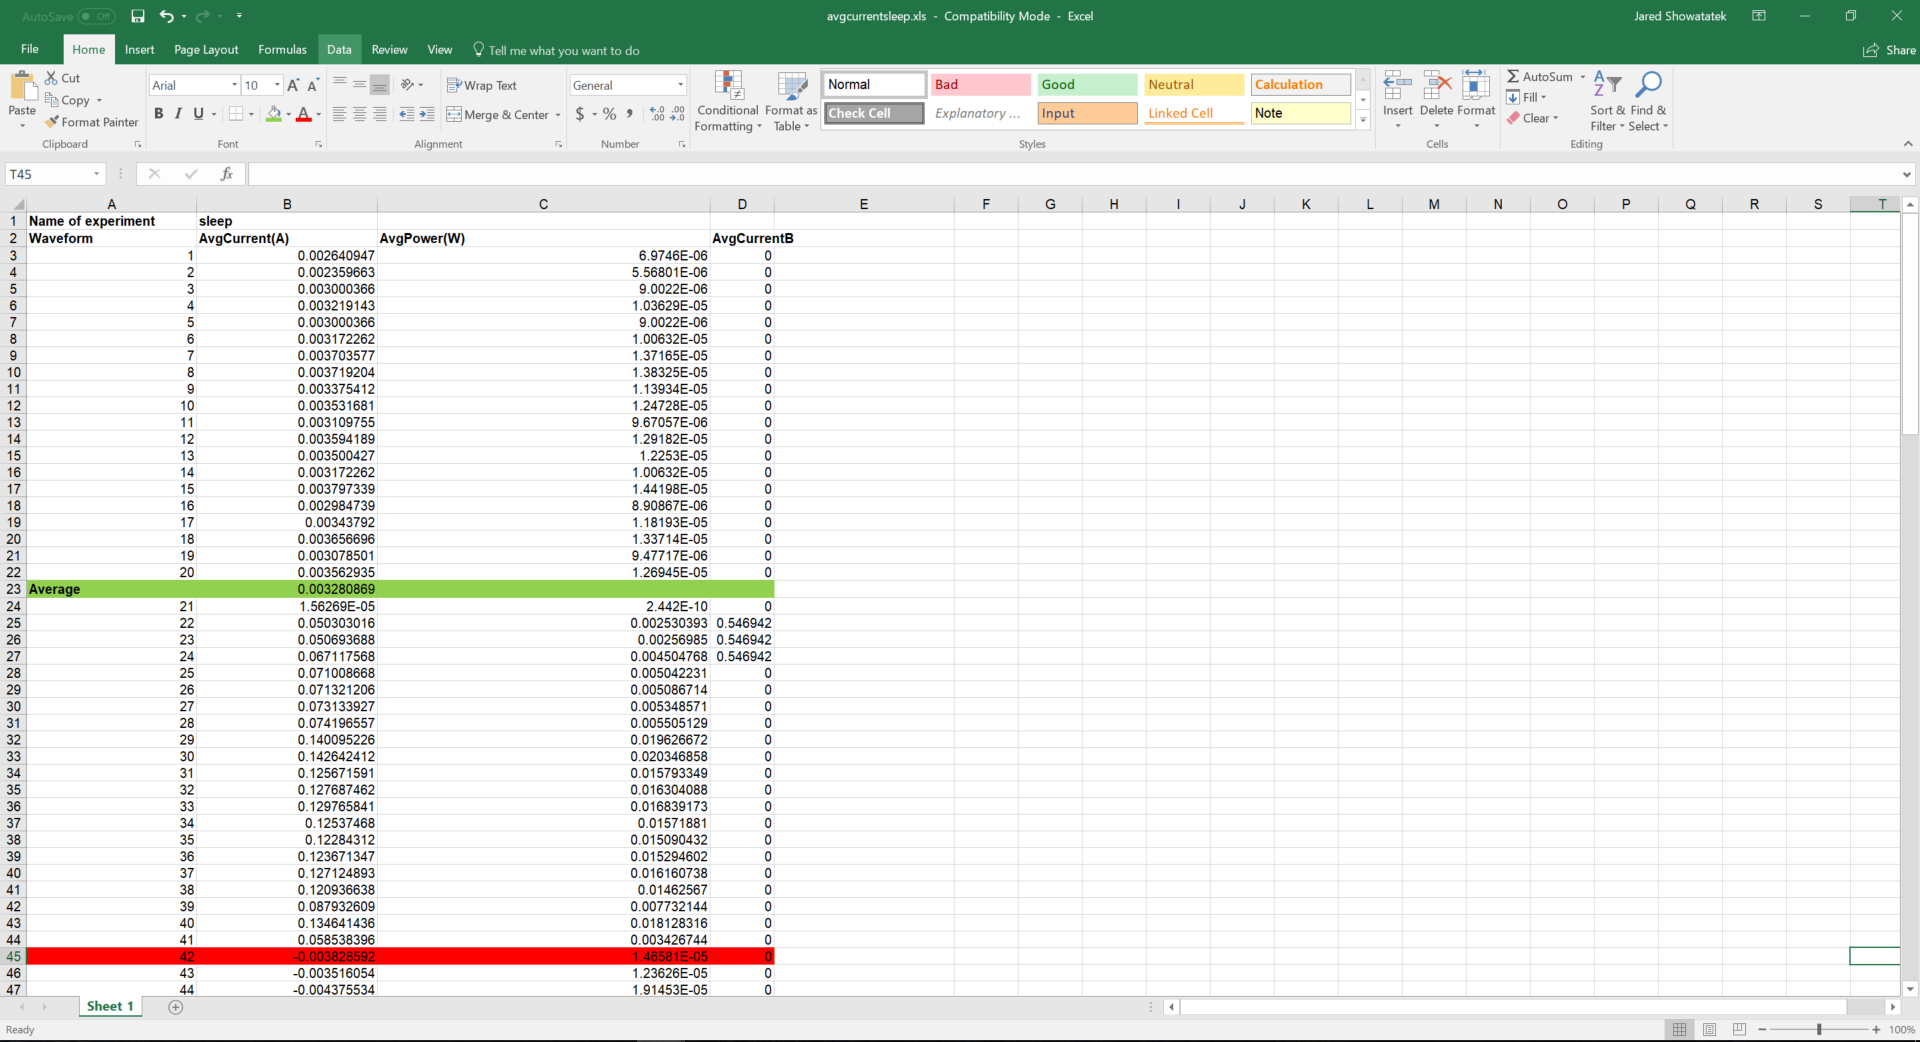
\includegraphics[width=16 cm]{Project_Report/Images/sleep.PNG}
\caption{The data from the deepsleep measurements}
\label{fig:deepsleep}
\end{figure}















\newpage
 \chapter{Energy Model}
 This chapter presents a simplified energy model based on the measurement and theory section. 
 \subsection{Data analysis}
 The first step in making an energy model of the GPS receiver is to analyze the data from the measurements and relating it to the theory. The theory section explains how the receiver operates between two distinct phases: acquisition and tracking. The two phases can be modelled in a state diagram. 
 
 
\begin{figure}[H]
\centering
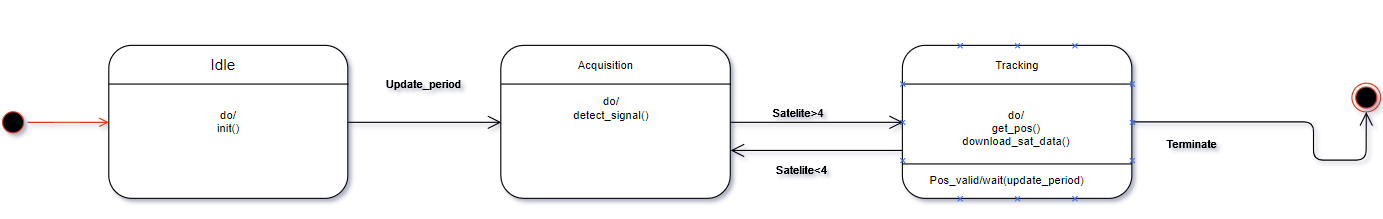
\includegraphics[width=16 cm]{Project_Report/Images/gps_basics.PNG}
\caption{The state diagram of a GPS receiver}
\label{fig:GPS reciever}
\end{figure}
 
 The trigger functionality from \ref{fig:WIFI_OFF} highlights when the receiver has a positional fix. We know from the theory, that the receiver switches to the tracking phase when it acquires a positional fix. This means that the GPS is in the tracking phase, the instant the trigger is set. The trigger functionality can't however, inform about later transitions because the receiver changes phases after it has a positional fix. The receiver does this to maintain its signal strength. The state diagram for the LoPy is an extension of \ref{fig:GPS reciever} with deepsleep and timeout. The extended state diagram is show in figure \ref{fig:GPS energymodel}
 
\begin{figure}[h]
\centering
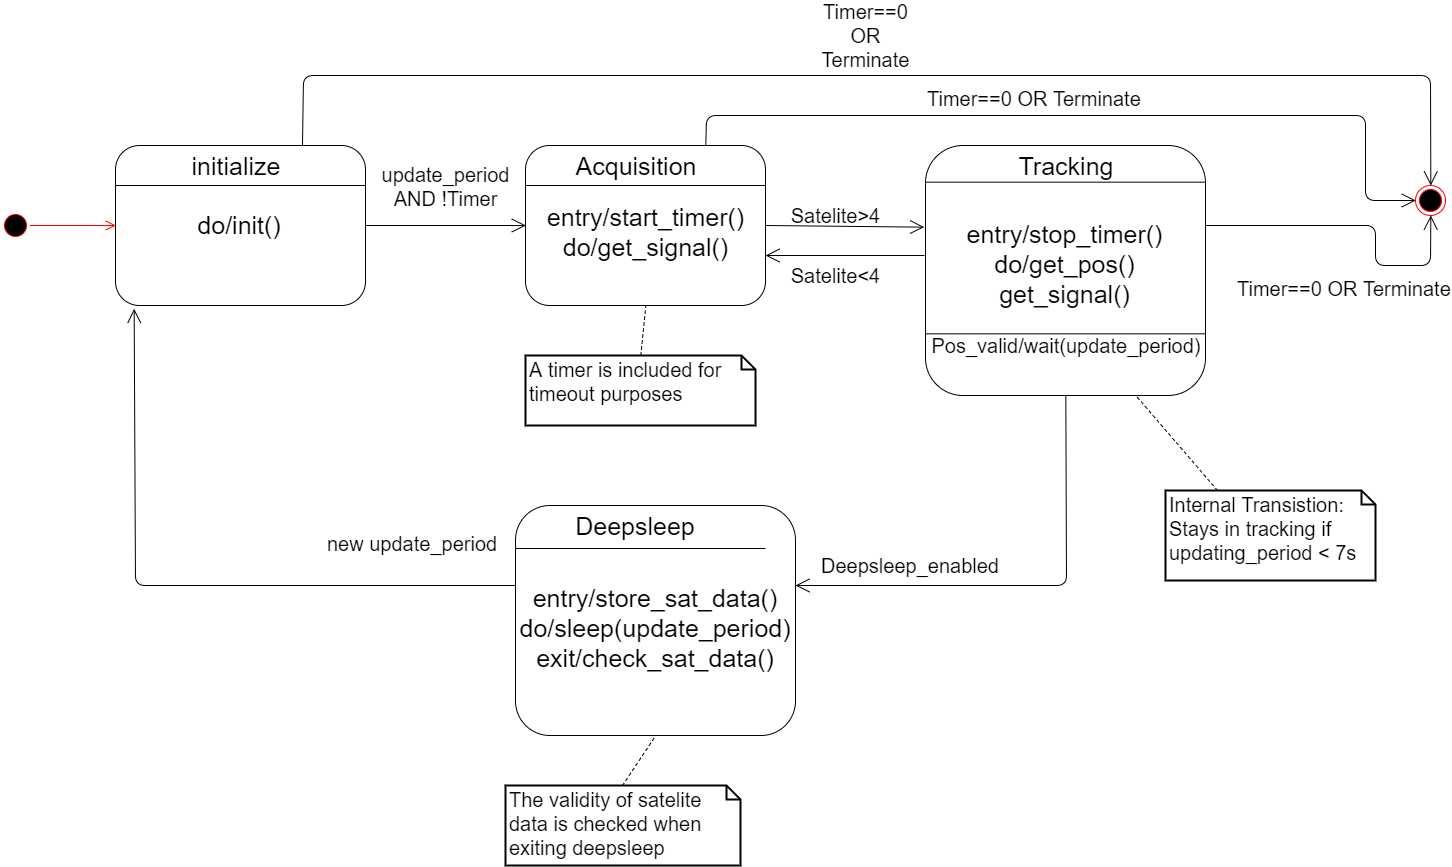
\includegraphics[width=15 cm]{Project_Report/Images/Energymodel.png}
\caption{The state diagram of the LoPy}
\label{fig:GPS energymodel}
\end{figure}
 
A table with the data of the current consumption right before and after the trigger is set, is generated in a acquisition and a tracking column respectively. The average of each column is calculated. A screenshot of the data along with the scatter plots for each column is shown in \ref{fig:average}
 
\begin{figure}[H]
\centering
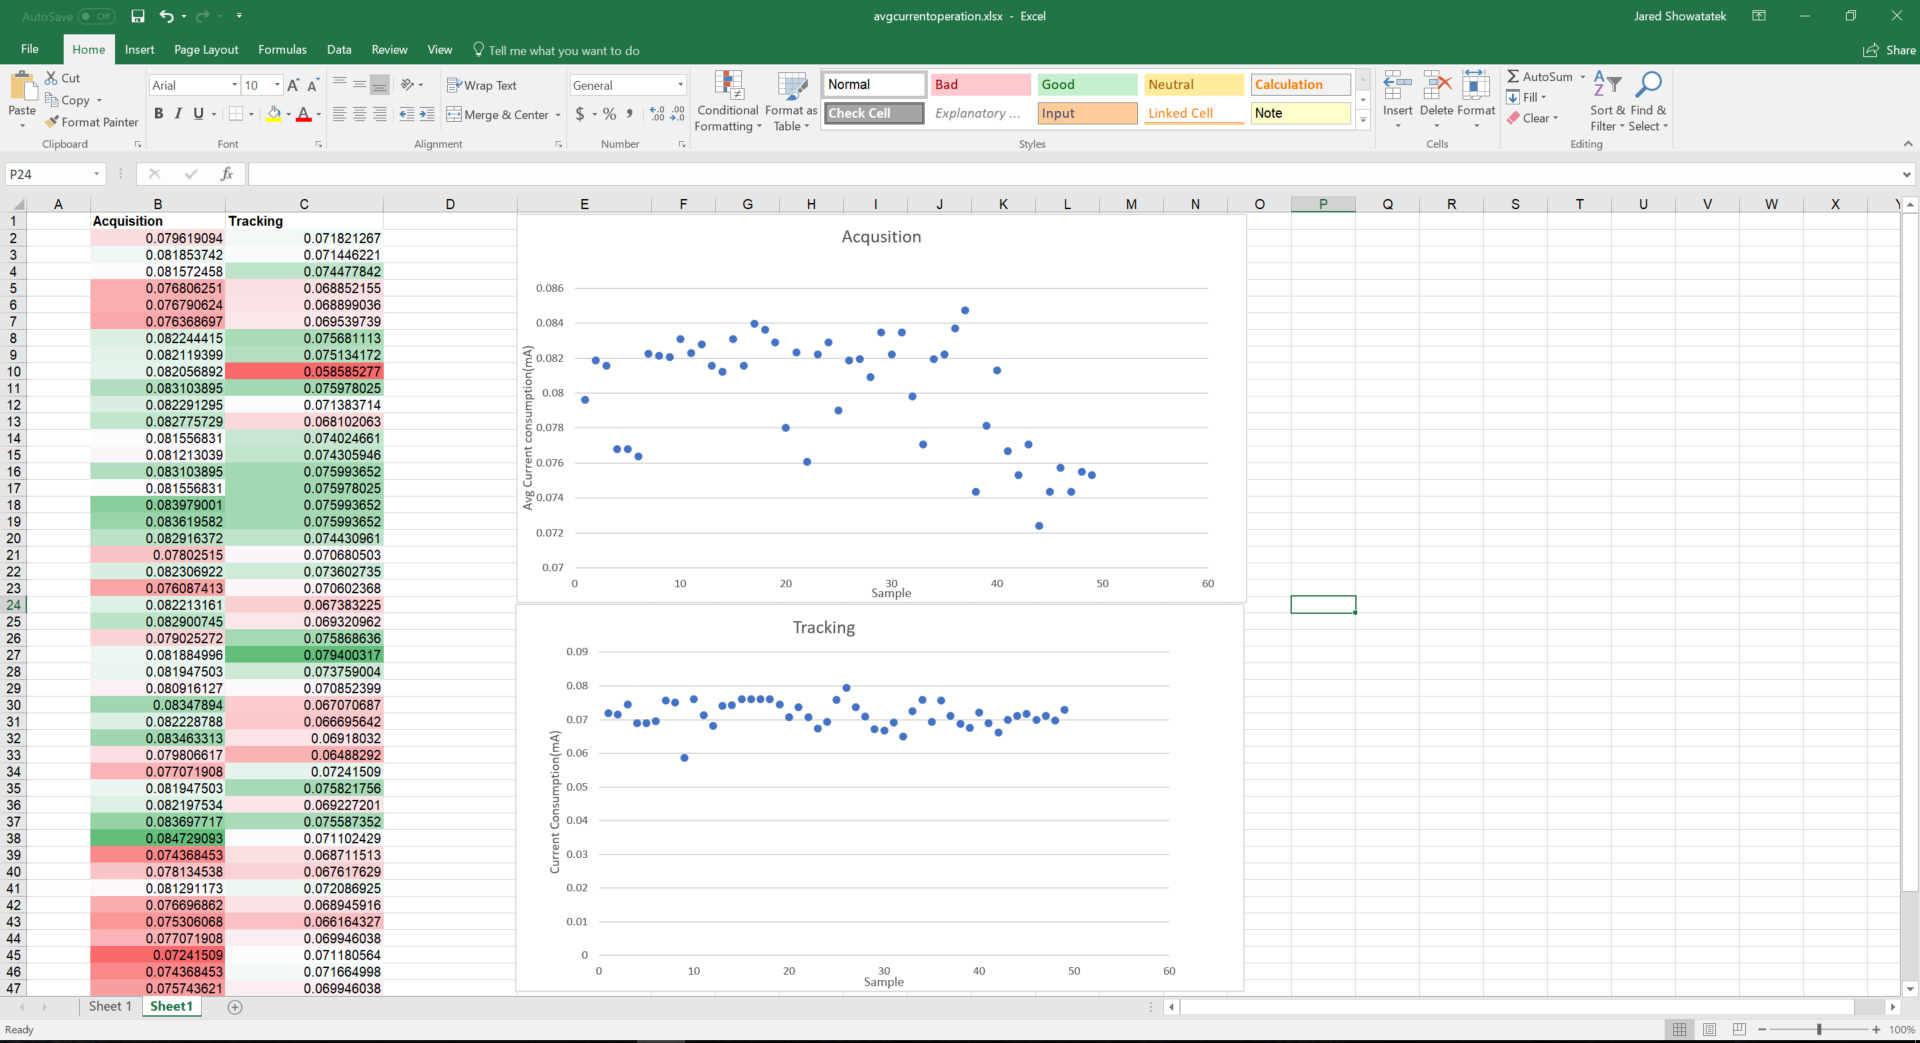
\includegraphics[width=15 cm]{Project_Report/Images/average.PNG}
\caption{The average values for acquisition and tracking phase }
\label{fig:average}
\end{figure}
 
 Average value of the acquisition and tracking phase is calculated to 80 mA and 72 mA respectively. \ref{fig:average} shows how the current consumption is decreasing in both of the states in the later measurements. The schematics from \ref{fig:LoPy_Schematic} shows that the LoPy is using a LiPo battery for voltage supply. Rechargeable batteries  tend to have a discharge curve, which means that the battery voltage changes during discharge. This affect might be the cause of the deviating voltage values in the later measurements. 
 
 The average values are compared with the features from the datasheet \cite{L76}. The datasheet state, that it should be a 7 mA difference between the acquisition and tracking phase. This seems to validate the measurements, which shows a decreasing in current consumption from 80 mA to 71 mA after a positional fix.   
 
 
\subsection{The model}
 
 
The python script in appendix \ref{Appendix:make_energy_model.py} use a simplified energy model to calculate the energy consumption over a fix period.
A fix period is defined as the duration the microcontroller use to acquire a fix from deepsleep:

\begin{equation}
E_{fixperiod} = P_{fixperiod}*T_{fixperiod}
\end{equation}
During a fix period, the microcontroller transitions between the states in figure \ref{fig:GPS energymodel}. The total energy consumption $E_{fixperiod}$ can then be written as the sum of the energy of each state:

\begin{equation}
E_{fixperiod} = P_{Idle}*T_{Idle} + P_{Acquisition}*T_{Acquisition} + P_{Tracking}*T_{Tracking} + P_{Deepsleep}*T_{Deepsleep}
\end{equation}
\begin{equation}
T_{Deepsleep} = {T_fixperiod} - {T_idle} - {T_Acquisition} - {T_Tracking}
\end{equation}
$T_ {Acquisition}$ depends on the last fix which is given by the $fix_period$.
The total energy consumption over a duration t is given by the energy consumption of a fix period multiplied by the number of periods during the total duration t.

\begin{equation}
 E_{total} = E_{fixperiod}* \frac{t}{fixperiod}
\end{equation}

Table \ref{Table:data for the energy model} shows the data that is used in the python script. The power is plotted in a pie diagram in figure \ref{fig:powerconsumption}
\begin{table}[h!]
\begin{center}
 \begin{tabular}{||c c c||} 
 \hline
  State & Time(s) & Power(W) \\ [0.5ex] 
 \hline\hline
  Idle & 5 & 10.201 \\ 
 \hline
 Acquisition & 1/30/35 & 6.4 \\
 \hline
 Tracking & 1 & 5.0 \\
 \hline
 Deepsleep &  & 0.01 \\
 [1ex]
 \hline
\end{tabular}
\end{center}
\caption{Data that is used for the energy model}
\label{Table:data for the energy model}
\end{table}

\begin{figure}[H]
\centering
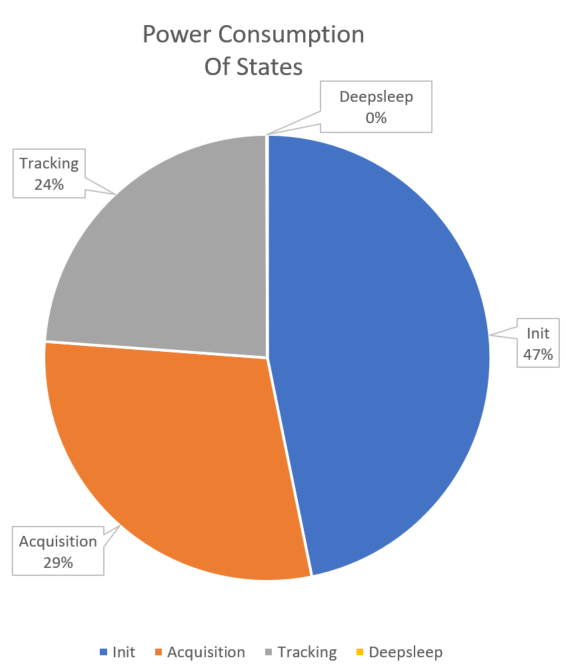
\includegraphics[height=7.5cm]{Project_Report/Images/powerconsump.PNG}
\caption{The pie diagram of the power in table \ref{Table:data for the energy model}}
\label{fig:powerconsumption}
\end{figure}

The values used for time in acquisition, depends on the validity of satellite data. The times that are given in table \ref{Table:data for the energy model} is from the specification \cite{L76}.
The python scripts generates an Excel sheet with the energy consumption for measuring the energy consumption of different fix periods over different durations. The data is given in table \ref{Table:energy}

\begin{table}[h!]
\begin{center}
 \begin{tabular}{||c c c c c c||} 
 \hline
 & Duration & & & & \\
 \hline
  & 60s & 1 Hour & 1 day & 30 days & 1 year \\
  Update Period & & & & &  \\[0.5ex] 
 \hline\hline
  1s & 0.3108 & 18.648 & 447.552 & 13426.6 & 163356 \\ 
 \hline
  10s & 0.278236 & 16.69414 & 400.6594 & 12019.78 & 146240.7 \\
 \hline
  60s & 0.046573 & 2.794357 & 67.06456 & 2011.937 & 24478.56 \\
 \hline
  1800s & -1 & 0.107065 & 2.569565 & 77.08696 & 937.8913 \\
  \hline
  3600s & -1 & 0.060733 & 1.457583 & 43.72748 & 532.0177 \\
  \hline
  14399s & -1 & -1 & 0.623615 & 18.70845 & 227.6195 \\
  \hline
  14400s & -1 & -1 & 1.708834 & 51.26501 & 623.7243\\
  \hline
  15551700s & -1 & -1 & -1 & -1 & 126.6047 \\
  \hline
  15552000s & -1 & -1 & -1 & -1 & 126.668 \\[1ex]
 \hline
\end{tabular}
\end{center}
\caption{Table displaying the energy consumption over different durations and update periods}
\label{Table:energy}
\end{table}

An invalid valid of -1 is given for update periods that are larger then the duration. 14400(4 hours) is the limit for the validity of the ephemeris. Having a update frequency 4 hours makes the validity of  ephemeris invalid, and makes the receiver spend 30 seconds instead of 1 second in the acquisition state. The benefit of having an updating period that is less than 4 hour, instead of just over 4 hours is shown in the table \ref{Table:energy}. The table shows that this strategy will save  $623.72 - 227.61 = 396.11 J$ over a year. A similar analysis is made for the Almanac. 15551700s(179 days) is the limit for the validity of the Almanac. But it isn't a noteworthy reduce of energy over a year:  $126.6047 - 126.668$. This is because of the small time penalty that is associated with an invalid Almanac versus just an invalid  ephemeris. A plot of the energy consumption is shown in figure \ref{fig:energyconsumption}

\begin{figure}[H]
\centering
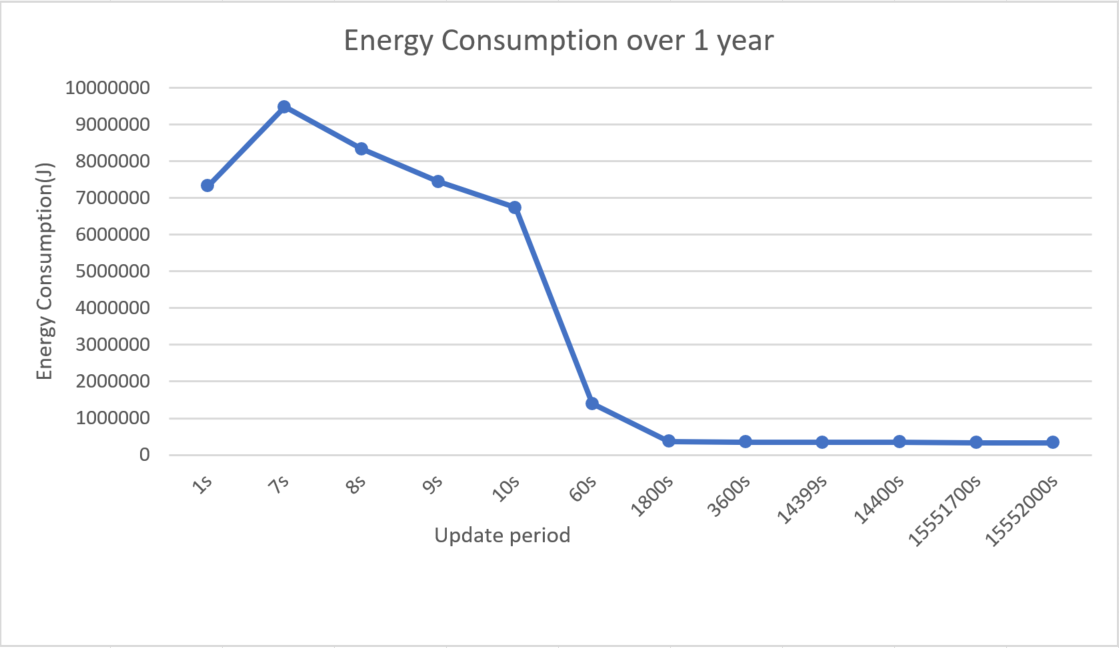
\includegraphics[height=7.0cm]{Project_Report/Images/energyconsumption.PNG}
\caption{The plot of table \ref{Table:energy}}
\label{fig:energyconsumption}
\end{figure}


It is possible to find the limiting updating period for when its more beneficial in terms of energy savings, to have an update frequency under 14400 versus over. The program in \ref{code:limit} uses the data from the energy model to find the limit updating frequency. The result from the execution of the program is shown in \ref{fig:limit}. 



\lstset{language=Python}          % Set your language (you can change the language for each code-block optionally)
\begin{lstlisting}[frame=single, caption= Code used for finding the beneficial limit]  % Start your code-block

    temp    =   Energy_consumption[4][5]
    optimal     =   Energy_consumption[4][6]
    fix_o = 14400

    while(temp<optimal):  
        T_sleep = fix_o - T_wake - 30 - T_track
        optimal = (P_sleep*T_sleep + P_wake*T_wake + P_acq*T_acq + P_track*T_track)*t[4]/fix_o
        print(optimal)
        fix_o = fix_o + 1

    print("Limit updating :",fix_o)
\end{lstlisting}
\label{code:limit}


\begin{figure}[H]
\centering
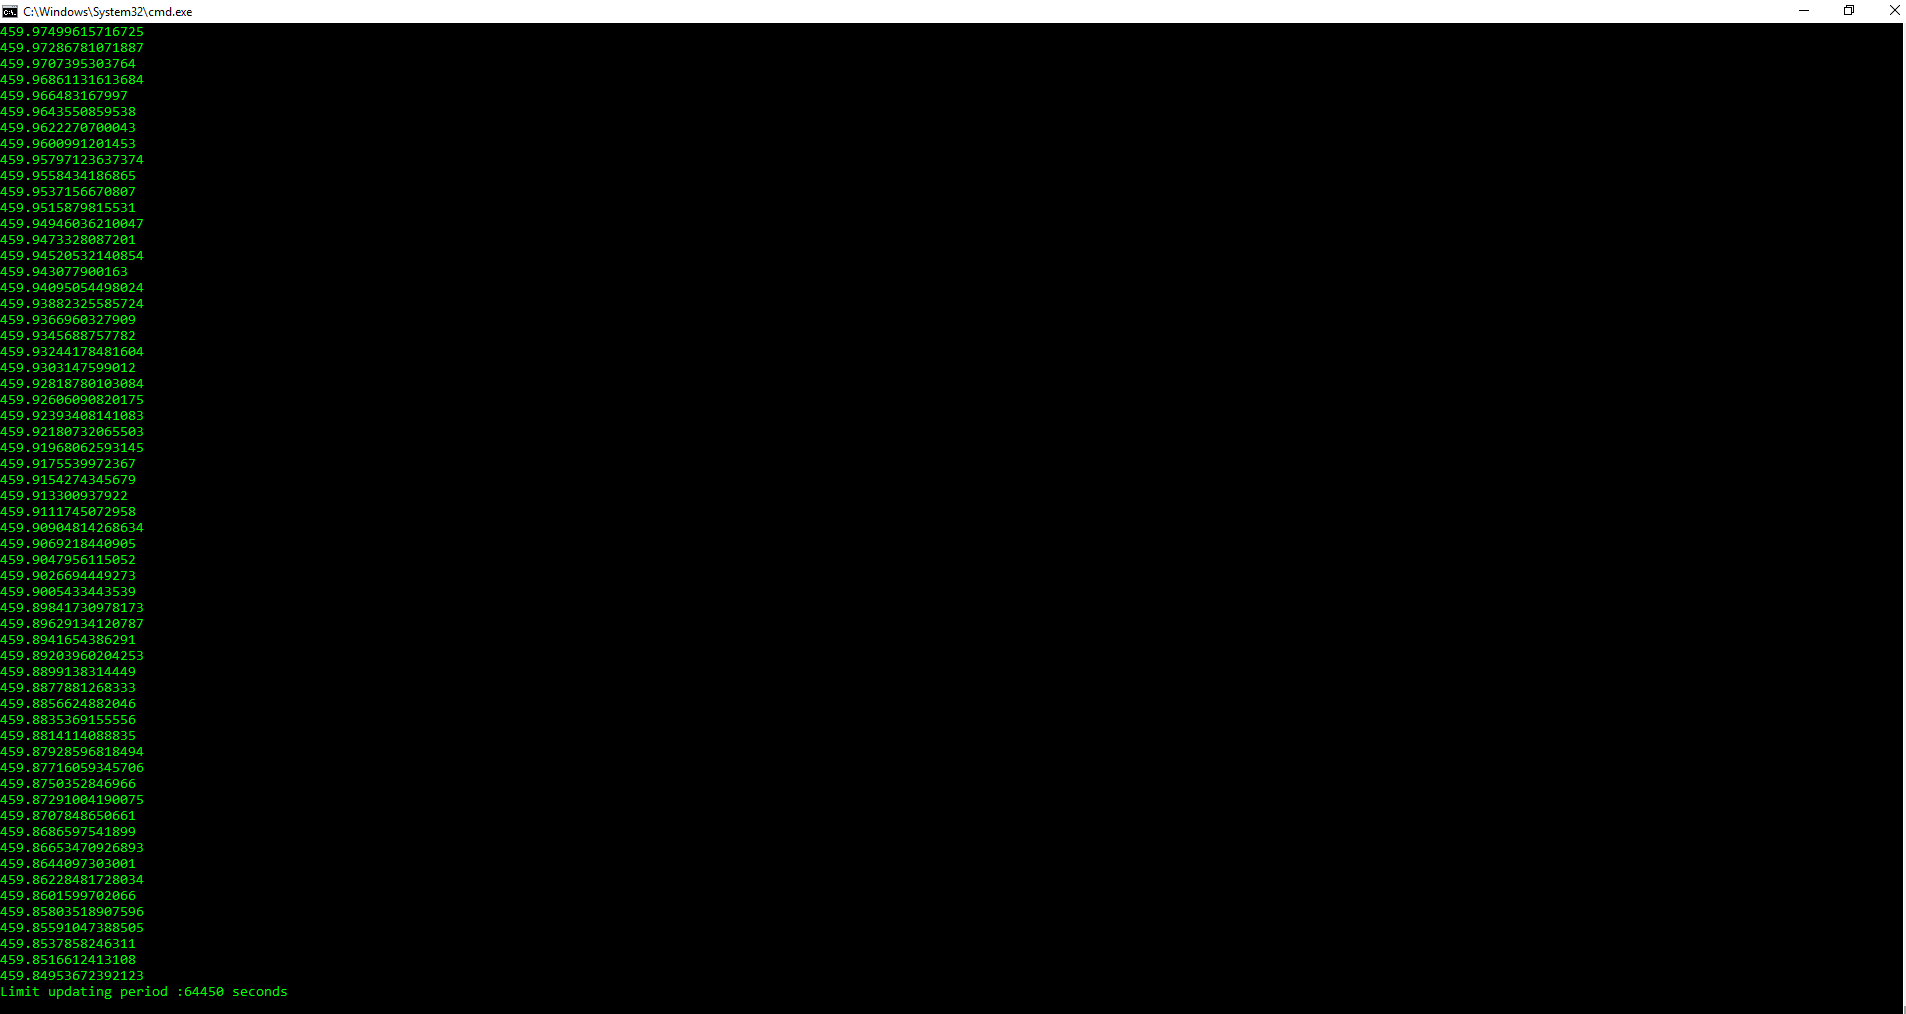
\includegraphics[height=8.0cm]{Project_Report/Images/limit.PNG}
\caption{A screenshot of the execution of the program code in \ref{code:limit}}
\label{fig:limit}
\end{figure}

It is therefore better to have an updating period of just under 4 hours versus having an longer updating period up to 64440 seconds. 



\newpage
\chapter{Discussion and conclusion}


% Bibliography - edit references.bib and use the \cite command in text
\bibliographystyle{plain}
\bibliography{Content/references.bib}
\begin{appendices}
\chapter{C027.cpp}
\begin{lstlisting}
#include "mbed.h"
#include "C027.h"
#include "rtos.h"

int power= 0;
char order= 'O';
int BAUDRATE=9600;
int timer;
int MEASURE_TIME= 1000000000;
C027 devkit;
DigitalOut trigger(D0);

void serialhandler(){
    //devkit.gpsPower(true);
    
    // open the gps serial port
    Serial gps(GPSTXD, GPSRXD);
    gps.baud(BAUDRATE);
    
    // open the PC serial port and (use the same baudrate)
    Serial pc(USBTX, USBRX);
    pc.baud(BAUDRATE);
    //devkit.gpsPower(true);
    while(1){
        if(pc.readable()){
            order = pc.getc();
            if(order=='D' && power){
                devkit.gpsPower(false);
                timer= MEASURE_TIME;
                power = 0;
                }
            else if(order=='E' && !power){
                devkit.gpsPower(true);
                timer= MEASURE_TIME;
                power= 1;
                }
            else if(order=='R'){
                    devkit.gpsReset();
                    timer = 0;
                    }  
        }
    if(gps.readable() && pc.writeable()){
        pc.putc(gps.getc());
        }
    }
}
void measure(){
     while(1){
     trigger.write(1);
     wait_ms(10);
     trigger.write(0); //Trekker utgangen ned
     wait_ms(10);
     timer --;
     while(timer<=0){
         wait_ms(1);
         }
    }
}
int main(){
    devkit.gpsPower(false);
    Thread thread_serial;
    Thread thread_measure;
    
    thread_measure.start(measure);
    thread_serial.start(serialhandler);
   while(1){}
    return 0; }
\end{lstlisting}
\label{Appendix:C027.Cpp}


\chapter{L76GNSS.py}
\begin{lstlisting}
from machine import Timer
import time
import gc
import binascii

class L76GNSS:
    STANDBY = bytes( [0x24,0x50,0x4D,0x54,0x4B,0x31,0x36,0x31,0x2C,0x30
    ,0x2A,0x32,0x38,0xD,0xA])
    GLONASS = bytes( [0x24,0x50,0x4D,0x54,0x4B,0x33,0x35,0x33,0x2C,
    0x30,0x2C,0x31,0x2A,0x33,0x36,0xD,0xA]) 
    COLD_START = bytes( [0x24,0x50,0x4D,0x54,0x4B,0x31,0x30,0x34,0x2A,
    0x33,0x37,0xD,0xA])
    PERIODIC_MODE = bytes( [0x24,0x50,0x4D,0x54,0x4B,0x32,0x32,0x35,
    0x2C,0x32,0x2C,0x33,0x30,0x30,0x30,0x2C,0x31,0x32,
    0x30,0x30,0x30,0x2C,0x31,0x38,0x30,0x30,0x30,0x2C,
    0x37,0x32,0x30,0x30,0x30,0x2A,0x31,0x35])

    GPS_I2CADDR = const(0x10)

    def __init__(self, pytrack=None, sda='P22', scl='P21', timeout=None):
        if pytrack is not None:
            self.i2c = pytrack.i2c
        else:
            from machine import I2C
            self.i2c = I2C(0, mode=I2C.MASTER, pins=(sda, scl))

        self.chrono = Timer.Chrono()

        self.timeout = timeout
        self.timeout_status = True

        self.reg = bytearray(1)
        self.i2c.writeto(GPS_I2CADDR, self.reg)
        self.fix = 0
        self.first_fix=0
        self.timestamp= 0
        self.gpgga_s= ''

        self.lat_d = 0
        self.lon_d = 0

    def write_gps(self,data,wait=True):
        print(data)
        self.i2c.writeto(GPS_I2CADDR, data)
        if wait:
             self.wait_gps()    
    def wait_gps(self):
        count = 0
        time.sleep_us(10)
        while self.i2c.readfrom(GPS_I2CADDR, 1)[0] != 0xFF:
            time.sleep_us(100)
            count += 1
            if (count > 500):  # timeout after 50ms
                raise Exception('Pytrack board timeout')


           
    def _read(self):
        self.reg = self.i2c.readfrom(GPS_I2CADDR, 64)
        return self.reg
    def _set_time(self):
        print('_set_time')
        self.timestamp = self.gpgga_s[1]
        print('timestamp set',self.timestamp)

    def _convert_coords(self):
        lat = self.gpgga_s[1]
        lat_d = (float(lat) // 100) + ((float(lat) % 100) / 60)
        lon = self.gpgga_s[3]
        lon_d = (float(lon) // 100) + ((float(lon) % 100) / 60)
        if self.gpgga_s[2] == 'S':
            lat_d *= -1
        if self.gpgga_s[4] == 'W':
            lon_d *= -1
        return(lat_d, lon_d)

    def get_fix(self):
        temp_fix= self.gpgga_s[6]
        self.fix = int(temp_fix)

    def coordinates(self, debug=False):
        lat_d, lon_d, debug_timeout = None, None, False
        if self.timeout != None:
            self.chrono.reset()
            self.chrono.start()
        nmea = b''
        while True:
            if self.timeout != None and self.chrono.read() 
            >= self.timeout:
                self.chrono.stop()
                chrono_timeout = self.chrono.read()
                self.chrono.reset()
                self.timeout_status = False
                debug_timeout = True
            if self.timeout_status != True:
                gc.collect()
                break
            nmea += self._read().lstrip(b'\n\n').rstrip(b'\n\n')
            gpgga_idx = nmea.find(b'GPGGA')
            if gpgga_idx >= 0:
                gpgga = nmea[gpgga_idx:]
                e_idx = gpgga.find(b'\r\n')
                if e_idx >= 0:
                    try:
                        gpgga = gpgga[:e_idx].decode('ascii')
                        print (gpgga)
                        self.gpgga_s = gpgga.split(',')
                        print(self.gpgga_s)
                        self.get_fix()
                        if(self.fix >0):
                            self.lat_d, self.lon_d = self
                            ._convert_coords(self.gpgga_s)
                    except Exception:
                        pass
                    finally:
                        nmea = nmea[(gpgga_idx + e_idx):]
                        gc.collect()
                        break
            else:
                gc.collect()
                if len(nmea) > 4096:
                    nmea = b''
           # time.sleep(0.1)
        self.timeout_status = True
        if debug and debug_timeout:
            print('GPS timed out after %f seconds' % (chrono_timeout))
            return(None, None)
        else:
            return(lat_d, lon_d)


\end{lstlisting}
\label{Appendix:L76GNSS.py}
\end{appendices}




\end{document}
